% ---- Chicago Thesis Style ---- %
%\documentclass[truedoublespace]{ccw_chithesis}
\documentclass[singlespace]{ccw_chithesis}
\usepackage{amssymb}
\usepackage{url}
\usepackage{graphicx}
\usepackage{multicol}
\usepackage{longtable}
\usepackage{hyphenat}
\usepackage{array}
\usepackage{color}
\usepackage{algorithm}
\usepackage{algorithmic}

\renewcommand{\algorithmicrequire}{\textbf{Input:}}
\renewcommand{\algorithmicensure}{\textbf{Output:}}

\begin{document}

% ---- Chicago Thesis Style ---- %
\title{A Resource Management Model for VM-Based Virtual Workspaces}
\author{Borja Sotomayor Basilio}
\department{Computer Science}
\division{Physical Sciences}
\degree{Master of Science}
\date{Draft as of \today}
\maketitle

\begin{abstract}
Virtual workspaces provide an abstraction for dynamically deployable execution environments on a Grid. For this abstraction to be effective, it must be possible to provide on-demand software environments and enforceable fine--grained resource allocations for these workspaces. Virtual machines are a promising vehicle to realize the virtual workspace abstraction, as they allow us to instantiate a precisely defined virtual resource, configured with desired software configuration and hardware properties, on a set of physical resources.

In this paper, we describe a model of virtual machine provisioning in a Grid environment that allows us to define such virtual resources and instantiate them on a physical Grid infrastructure. Our model focuses, firstly, on providing users with an accurate representation of virtual resources. To accomplish this, the overhead resulting from instantiating and managing virtual resources is scheduled at the same level as virtual resources, instead of being deducted from a user's resource allocation. Secondly, our model also focuses on efficiently managing virtual resources by reducing the amount of overhead.

We argue that this model, compared to resource management models that rely on the job abstraction for remote execution, enables resource providers to accurately provision resources to users, while using their physical resources efficiently. We show experimental results that demonstrate the benefits of this model both from the resource provider's and the user's perspective, in two common resource management scenarios for virtual workspaces: advance reservations and batch--style submissions.
\end{abstract}

% More acknowledgements will be added in the final draft of the thesis
\acknowledgments
This work was supported by NSF CSR award \#527448 and in part, by the
Mathematical, Information, and Computational Sciences Division
subprogram of the Office of Advanced Scientific Computing Research,
SciDAC Program, Office of Science, U.S. Department of Energy, under
Contract W{}-31{}-109{}-ENG{}-38

\tableofcontents
\listoffigures
\listoftables

\renewcommand{\chaptername}{Section}

\mainmatter

\chapter{Introduction}
\label{cha:introduction}
Currently, execution management on Grid systems is commonly performed through the use of the \emph{job} abstraction, where users submit an executable file furnished with metadata, such as a list of computational resources required by the job, to a resource provider that, in turn, will schedule the job according to local policies. In most grid deployments today, users only have limited control over the resource platform on which computations are performed. In particular, two types of control are often lacking:

\begin{description}
\item[Availability and quantity of resources:] Users are limited to requesting coarse-grained resource allocations, such as number of CPUs, disk space, and memory. \emph{Finer-grained allocations}, such as percentage of a CPU, disk read/write speeds, and network bandwidth cannot be specified. In terms of availability, assuming no advance reservation capabilities, users have no control over the starting and ending time of their jobs, which will depend instead on local scheduling policies.
\item[Software environment:] Users are limited to the software environments available in the resource providers, which might not provide all the necessary dependencies (such as libraries) to run their jobs. Users may find that resource providers, who have to meet the needs of diverse communities, are unable or unwilling to install the software they need to run their jobs, limiting their choice of providers. Additionally, resource providers generally run jobs in a restricted execution environment, precluding the execution of any code requiring administrative privileges for all or part of its work.
\end{description}

Although these limitations are acceptable for a wide variety of computations, they can be a barrier for many others. Control over resource availability is particularly important for deadline{}-sensitive applications, in which a resource needs to be made available in response to a specific event, such as data becoming available from a sensor, a class starting at a specific time, and input from a human client. Although such control can be provided via reservation mechanisms, access to these reservations are carefully rationed by resource providers because of their negative impact on resource utilization. The lack of control over software configuration can be a barrier to the use of remote resources and providing more control over this aspect can increase demand for remote computing resources.

With these requirements in mind, Keahey et al. \cite{VirtualWorkspaces05} defined \emph{virtual workspaces} (VWs), a construct that allows clients to negotiate the creation of a virtual computing resource with a specified software environment and resource allocation. The workspace interface allows a remote client to negotiate and manage a virtual resource allocation securely using Web Services{}-based protocols for state access and management \cite{ModelingState05}. Virtual machines (VMs), such as Xen \cite{xen} and VMware \cite{vmwareweb}, with their isolation and virtualization properties, provide a
particularly promising platform for workspaces.

In this paper, we present and evaluate a resource management model for virtual workspaces designed to enable accurate and efficient creation of VM{}-based virtual workspaces. We constraint most of our discussion of resource management to the resource dimension of time or \emph{availability}, leaving more exhaustive investigations of other dimensions (such as memory, CPU, network bandwidth, etc.) to future work. Thus, we understand \emph{accuracy} to mean that a request to create a virtual workspace at a particular time $t$ (either immediately, or in the future) is satisfied at that time $t$, not later. By \emph{efficient}, we mean that the overheads incurred by the server(s) that process requests for virtual workspace creation are low. As we shall see, accuracy and efficiency are greatly affected by the size of virtual machine images required to run virtual workspaces, which can be large. 

We present real and simulated experimental results that use the resource management techniques presented in this paper to schedule virtual workspaces. These results show that, by annotating virtual machine images with descriptive metadata, a scheduler will be capable of better managing the overhead of creating a virtual workspace, resulting in improved accuracy of deadline--sensitive deployments. Furthermore, our experiments show that, by using a set of image prefetching and reuse techniques, greater efficiency can be achieved, reducing the time required to process requests on a best--effort basis. Our experiments will also explore workloads that combine deadline--sensitive and best--effort requests, and how resource management mechanisms that are part of most virtual machine systems can improve utilization of physical resources.

The rest of this paper is structured as follows. We begin, in Section~\ref{cha:background}, by providing some background on Grid Computing and Virtual Workspaces. Next, Section~\ref{cha:scenarios} presents the resource management scenarios
that motivate our virtual workspaces work, followed by a description, in Section~\ref{cha:problem}, of the specific problem we address in this work. Section~\ref{cha:virtualresources} explains our virtual resource model, Sections~\ref{cha:design}  and~\ref{cha:impl} describe the design and implementation, respectively, of our VW scheduling system, and Section~\ref{cha:experiments} presents our experimental results. Finally, Section~\ref{cha:related} discusses related work, and Section~\ref{cha:conclusions} presents our conclusions and future work.



\chapter{Background: Virtual Workspaces}
\label{cha:background}
\label{sec:vw}

In Section~\ref{cha:introduction}, we introduced the concept of \emph{virtual workspaces}. In this section we provide a more in--depth description of the term virtual workspace, a discussion of why virtual machines are a promising vehicle for virtual workspaces, and approaches to implementing workspaces, including the Globus Toolkit 4 Workspace Service.

Virtual workspaces were first introduced by Keahey et al.\cite{VirtualWorkspaces05} as an abstraction for execution environments that can be deployed on a grid. This construct does not arise as a replacement for other execution management approaches, such as the widespread \emph{job} abstraction. Rather, it is a more general abstraction adequate for use cases requiring \emph{dynamic} and \emph{secure} deployment of execution environments (see Section~\ref{cha:scenarios}). This deployment can be dynamic if the user needs the execution environment to be created and destroyed on--demand, and it must be secure because both the software environment contained in the workspace and the user creating/managing/accessing the workspace must be trustworthy.

The two distinguishing aspects of virtual workspaces are:

\begin{description}
\item[Environment definition] or \emph{Quality of Life}: Workspaces provide an execution environment meeting all the software requirements of a user.
\item[Resource allocation] or \emph{Quality of Service}: All the resources the workspace needs to function correctly (CPU, memory, disk, bandwidth) must be provisioned and guaranteed during an agreed--upon availability period, allowing for dynamic renegotiation to reflect changing requirements and conditions.
\end{description}

The idea of on--demand creation and management of execution environments is not a new one, and there are multiple approaches to this problem, such as cluster node imaging (e.g. Cluster--on--Demand \cite{codweb}), configuration management (e.g. bcfg2 \cite{bcfg2web}), or package management (e.g. Pacman \cite{pacmanweb}). However, these approaches are not adequate for the stated goals. From the quality of life perspective, cluster node imaging and configuration management limit the software environments the user can choose. From the quality of service perspective, deploying hard drive images to cluster nodes requires a preparation time during which those nodes will be unavailable, and package management takes a long time to install and configure all necessary packages to create a software environment. Furthermore, none of these approaches support enforceable fine--grained resource allocation.


\section{VM--based Virtual Workspaces}
\label{sec:vm}

The use of virtualization technologies \cite{vmbook} holds great potential for Grid Computing. Figueiredo et al.\cite{gridvm} outlined the following general advantages of using virtual machines in the context of Grid Computing:

\begin{description}
\item[Security and isolation:] Virtualization isolates the actions performed in one VM from other VMs running in the same physical machine. Thus, VMs add an extra layer that must be broken by malicious grid users before the performance of co--allocated VMs can be affected, and before physical resource integrity can be compromised.
\item[Customization:] Virtual machines can be customized with specific software and hardware requirements, without restarting physical nodes.
\item[Legacy support:] As a consequence of customization, virtual machines can be configured to replicate legacy software and hardware environments, enabling support of legacy code without affecting the software environment of users requiring newer software.
\item[Administrator privileges:] Users can be granted administrator privileges inside a virtual machine, since any malicious activity will be confined to the virtual machine, and will not affect the underlying physical machine.\footnote{Figueiredo et al. makes no reference to the fact that granting administrator privileges can enable malicious users to initiate attacks that require ``root'' access (such as a denial--of--service attack by flooding the network with packages, something which a non-privileged user user cannot do). Granting administrator privileges inside a virtual machine is, nonetheless, preferable to granting them on a physical machine, as system administrators can easily shut down malicious virtual machines without affecting any co--allocated virtual machines.}
\item[Resource control:] Virtual machines enable enforceable fine--grained resource allocations that can be specified when creating the virtual machine, but also modified during the virtual machine's runtime. The resource enforcement mechanisms of virtual machines allow administrators to limit the impact of a VM's resource consumption on other co--allocated virtual machines, and also enables fine--grained accounting of resource usage. 
\item[Site-independence:] Virtual machines are very loosely coupled to physical hosts, only requiring that a host have an adequate virtual machine monitor and sufficient resources to support its execution. This enables virtual machines to be instantiated in different sites, imposing fewer constraints on the physical configuration of the site. Furthermore, virtual machines can be seamlessly migrated from one site to another.
\end{description}

Quality of life and service in virtual workspaces can be enhanced by leveraging these advantages. Security, isolation, and resource control positively affect quality of service by guaranteeing that workspaces have enough resources (CPU, memory, etc.) to support their execution, while being isolated from the resource usage of other co--located workspaces. Site--independence can improve quality of service by increasing the pool of physical resources where a workspace can run, and enabling cross--domain load balancing of workspaces. Customization, legacy support, and administrator privileges provide the users with quality of life, by decoupling them from the software environment provided by a resource provider and enabling them to specify custom software environments inside a virtual machine.

Virtual machine (VM) technologies  are, thus, a promising vehicle for achieving high quality of life and service in virtual workspaces. In a VM--based virtual workspace, the software environment required by the user would be encapsulated inside a virtual machine, and resource allocations would be enforced by a virtual machine manager.

\section{Representation of VM--based Virtual Workspaces}
\label{sec:vwrepresentation}

\begin{figure}
  \begin{center}
    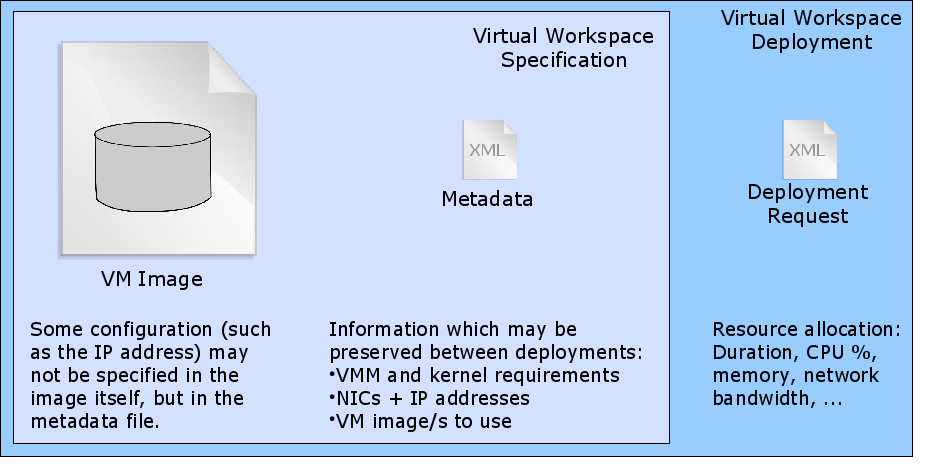
\includegraphics[width=0.85\textwidth]{figures/vw_representation.png}
    \caption{Virtual Workspace Representation}
	\label{fig:vwrepresentation}
  \end{center}
\end{figure}


A VM--based virtual workspace is composed of two elements \cite{VirtualWorkspaces05}, summarized in Figure~\ref{fig:vwrepresentation}, the \emph{VM image} and the \emph{workspace metadata}.

In a VM-based virtual workspace deployment, one or more virtual machines will be run. To instantiate a virtual machine, we need a \emph{disk image} with a runnable operating system and all the software required by the user. A VM image is composed of one or more disk images, representing the different disk partitions required by the virtual machines. Users could potentially provide their own VM images, or choose from a set of preexisting images made available by a resource provider.

Deployment--independent configuration information is factored out of the VM image and into an XML \emph{metadata file}. This approach allows workspaces to be described in terms of \emph{VM image templates}, generic reusable VM images with the system software and tools for some specific purpose (e.g. a worker node for an Open Science Grid cluster), but lacking all the configuration information specific to a particular type of deployment. This information, contained in the metadata file, is \emph{bound} to the VM image at runtime to produce an \emph{image instance}.

To illustrate the concept of image templates and why information in the metadata file is deployment--independent we present the following example:

\begin{enumerate}
\item A user wishes to deploy a virtual workspace representing an Open Science Grid (OSG) cluster with 100 worker nodes (for the purposes of this example, we will ignore the head node and focus only on the worker nodes). We assume that worker nodes differ only in their network configuration, and that the user wants to specify a single private IP address for each worker node manually (and not rely on other mechanisms, such as DHCP). Since each worker node will have a different network configuration, the user could prepare 100 worker node images, $W_1\ldots W_{100}$, that differ only in their network configuration. By using image templates and metadata files, the user only needs to provide a \emph{single} VM image $W$ and a metadata file $mf$ containing the network configuration of each of the worker nodes ($conf_1\ldots conf_{100}$).
\item When the virtual workspace is deployed, multiple copies of the image template are made, and each is bound to the configuration contained in the metadata file to produce runnable image instances (e.g. $W(conf_{42})=W_{42}$). Note that the image template is reusable, since a single copy of an image template can be used to yield multiple image instances.
\item Metadata file $mf$ can be reused for future deployments of a 100--node OSG cluster. In this sense, the configuration information contained in the metadata file is \emph{deployment--independent}.
\item In the future, the user wishes to deploy a 150--node cluster, using the same VM image $W$. Metadata file $mf$ cannot be used as it only includes configuration for 100 nodes. To deploy the new workspace, the user must create a new metadata file, $mf'$, with configuration information for all the nodes ($conf_1\ldots conf_{150}$). Similarly, if the user wishes to deploy the 100--node cluster but using network addresses different from the ones specified in $mf$, a new metadata file would also be required. Therefore, we consider that any configuration information that \emph{need not} change across deployments is deployment--independent. Furthermore, this example also shows how an image template can be reused not just in a single deployment (by using it to create multiple image instances) but across deployments, since all potentially mutable information is contained in the metadata file, not in the VM image.
\end{enumerate}

In Section~\ref{cha:design} we will explore optimizations that result from the reusability of image templates.

Finally, when a virtual workspace is deployed, we must also specify a \emph{deployment request} (also shown in Figure~\ref{fig:vwrepresentation}). This request is an XML document describing the resource
allocation required by the workspace, including both availability and hardware requirements (such as memory and
CPU\%). This information is \emph{deployment--dependent}, since resource allocation requirements generally vary across deployments (e.g., the user might be interested in performing CPU--intensive work in one deployment, and I/O--intensive work in another), and also during a deployment (to adapt to changing requirements and conditions).


\section{GT4 Workspace Service}

\begin{figure}
  \begin{center}
    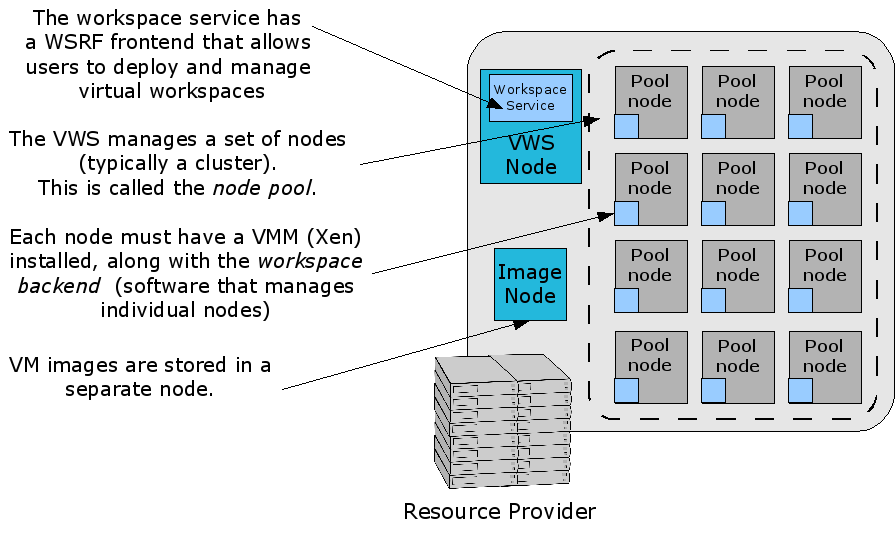
\includegraphics[width=\textwidth]{figures/vw_overview.png}
    \caption{Virtual Workspace Service}
	\label{fig:vwservice}
  \end{center}
\end{figure}


The GT4 Virtual Workspace Service \cite{vwsweb}, or VWS, which we extend in this work, allows authorized users to request the creation of VM--based virtual workspaces through a Web Services interface. This interface also allows users to monitor and control the virtual workspace. As of this writing, the VWS only supports single--node virtual workspaces and immediate reservations without the possibility of queueing or preemption (i.e. requests for which resources cannot be provisioned immediately  are rejected). Virtual machines are instantiated using the Xen Virtual Machine Monitor \cite{xen}, although others (such as VMWare \cite{vmwareweb}) could potentially be used.

Figure~\ref{fig:vwservice} shows the typical setup required by the VWS in the resource provider:

\begin{itemize}
\item A publicly accessible node, the \emph{VWS node}, hosts the Web Service frontend of the VWS.
\item A set of nodes, the \emph{node pool} are put under the control of the VWS. Virtual workspaces will be deployed on these nodes.
\item Each node in the node pool must have a virtual machine manager installed, along with the \emph{workspace backend}, a script that manages individual nodes and is invoked by the VWS when tasks need to be performed on nodes (such as starting and stopping virtual machines.
\item A separate node, the \emph{image node} acts as a repository for VM images. When a virtual workspace is deployed on the node pool, VM images are staged to the nodes from the image node.
\end{itemize}

In a typical interaction with the VWS, the following steps would take place:

\begin{enumerate}
\item A user wishes to deploy a virtual workspace. To do so, the user provides the location of the VM image (in either the image node or a third--party site), the workspace metadata, and the deployment request (as described in the previous section).
\item The VWS determines if there are enough resources immediately available to satisfy the request. If not, the request is rejected. Otherwise, the VWS initiates a transfer of the VM image to the nodes where that VM image will be used.
\item Once the image transfer is completed, the VWS uses the workspace backend to start the virtual machines for the requested workspace.
\item Information about the workspace, such as its status, the IP addresses assigned to the virtual machines, etc. are published through the Web Services interface, using WSRF Resource Properties.
\item Users can query these Resource Properties, and interact with their workspaces in the same way they would with a physical machine.
\item Users can also use the Web Services interface to control their workspaces (e.g. to stop them when they are done with their work)
\end{enumerate}



\chapter{Resource Management Scenarios}
\label{cha:scenarios}
Our work is motivated by a variety of use cases with quality of life and service requirements that can be met by virtual workspaces. For example:

\begin{description}
\item [Virtual labs:] A university wishes to teach a course on Parallel Programming, but lacks a cluster on which students can run their exercises, labs, etc. Even with a cluster in the university, the cluster administrator is unlikely to grant students complete control of the cluster during class hours. A virtual workspace can be created dynamically during the times when the course's labs are in session, providing students with an execution environment where they can do their exercises.
\item [Event-driven applications:] Applications requiring large amounts of computational resources when an event arrives (such as data arriving from an experiment) or emergency applications, such as flood modeling, require systems that can provision resources immediately, preempting any other work taking place on the computational resources. VM--based virtual workspaces could be used to meet the quality of service requirements of event--driven applications, thanks to their ability to reshape resource allocations dynamically and suspend and resume computations seamlessly.
\item [Batch jobs with strict software requirements:] Users who need to run batch--style jobs, but require very specific software environments (e.g., legacy environments) that system administrators may not be willing to provide as they have to take into account the software needs of all their users. Virtual workspaces can provide users with exactly the software environment they need to run their jobs.
\end{description}

Our goal is to arrive at a resource management model that meets the requirements of the above use cases. In particular, we concern ourselves here with \emph{availability}. Freeman et al. \cite{DBLP:conf/icsoc/FreemanKFRSW06} explored the protocols and enforcement methods along other resource dimensions, such as CPU and network bandwidth, highlighting the interdependencies that can arise between different resource dimensions. We leave a more exhaustive discussion of multi--dimensional resource management for future work.

Before discussing the different availability scenarios that arise in these use cases, and which will be the object or our investigations, we present the following definitions:

\begin{description}
\item[Agreement:]  We adopt the definition provided in the WS-Agreement specification~\cite{wsag}: \emph{``An agreement defines a dynamically--established and dynamically--managed relationship between parties. The object of this relationship is the delivery
of a service by one of the parties within the context of the agreement. The management of this delivery is achieved by agreeing on the respective roles, rights and obligations of the parties. The agreement may specify not only functional properties for identification or creation of the service, but also non-functional properties of the service such as performance or availability. [\ldots].''} In the context of our work, the two parties involved are a resource provider and a resource consumer (which we will refer to simply as the \emph{user}). The service to be provided is access to computational resources, and we focus on satisfying the availability requirements specified by the user.
\item[Availability period:] A period defined by agreed--upon events happening at any time while the agreement is valid. During this period of time, the resources requested by the user are guaranteed to be accessible.
\item[Agreement establishment time:] Precise instant in time in which a user establishes an agreement with the resource provider. The period during which the agreement is valid need not start at this time (e.g., an agreement for future use of resources)
\item[Event:] An occurrence that affects availability. Events can be received and processed automatically by a local resource manager, without any human intervention on the resource provider's side. They can arrive at any time, but are only guaranteed to be processed while the agreement is valid. Examples of events include:
\begin{itemize}
\item \emph{User request}: The user explicitly requests the start or termination of the availability period.
\item \emph{Asynchronous events}: The user defines an asynchronous event, such as arrival of data from an experiment, that must trigger the start of the availability period (e.g., because we need computational resources to analyze the data arriving from the experiment).
\item \emph{Timer events}: Events ocurring at a specific time as a consequence of a timer manager by a resource manager. This can include timers that set off the beginning of an availability period, or its duration. A scheduler will typically determine these times based on local policies, or on pre--agreed times.
\end{itemize}
\end{description}


\begin{figure}
  \begin{center}
    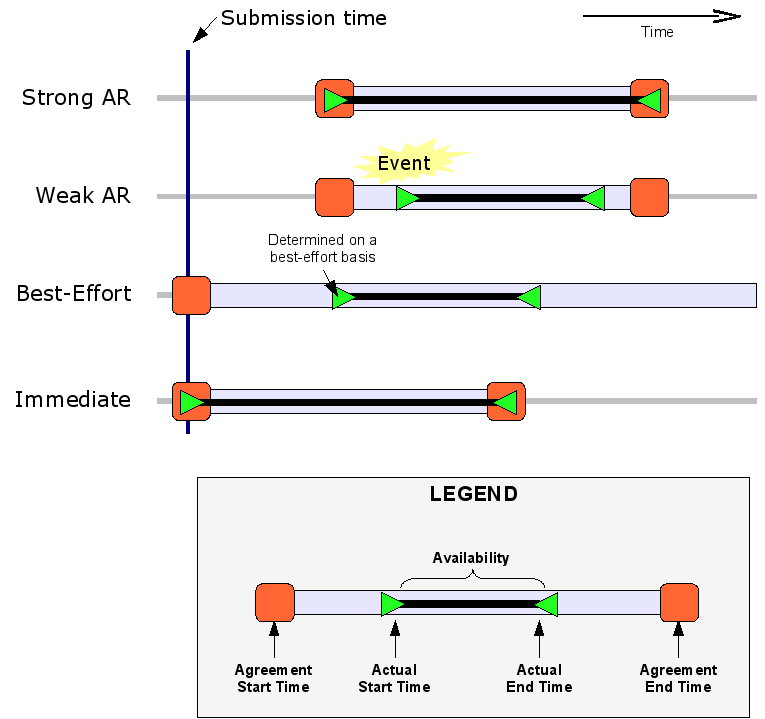
\includegraphics[width=\textwidth]{figures/availability.png}
    \caption{Availability scenarios}
    \label{fig:availability}
  \end{center}
\end{figure}

Depending on how strictly availability is defined, we encounter different \emph{availability scenarios}, which can be described with terms such as `advance reservations', `batch submissions', `best--effort scheduling', etc. Since these terms tend to be highly overloaded, throughout this text we will observe the following definitions (summarized in Figure~\ref{fig:availability}):

\begin{description}
\item[Closed Advance Reservation]: Availability in this case is clearly defined \emph{in advance} with pre--agreed start and end timestamps that coincide with the start and end of the agreement. Virtual workspaces for the \emph{Virtual Labs} use case, for example, will have specific start and end times (e.g. a lab that is taught from 2pm to 4pm).
\item[Open Advance Reservation]: In event--driven applications, availability requirements are loosely defined, since the user can only specify the availability period in terms of asynchronous events (and, possibly, also a window of time during which those events are likely to arrive). However, when that event is received, availability \emph{must} be guaranteed at exactly that time, and for the duration specified. Thus, this availability scenario is an advance reservation insofar as the resource requirements are known in advance, meaning the scheduler can take steps to  provision resources preemptively in case the start event arrives, but the exact start and end times are not. The Urgent Computing use case is an example of Open AR.
\item[Best--effort Reservation]: Similarly to Open AR, this availability scenario presents loosely defined availability requirements. The user agrees to have availability defined by the resource manager, which will provision resources on a best--effort basis, taking into account local policies regarding prioritization and quotas, and queueing requests if necessary. Batch jobs are an example of this availability scenario.
\item[Immediate Reservation]: In this case, availability requirements are not known until the time the resource request arrives and, once it arrives, resources must be  provisioned immediately. Unlike Open AR, the resource manager would have no way of preemptively provisioning resources for this kind of resources, and a request is rejected if resources cannot be  provisioned immediately. This scenario is, arguably, just a special case of Closed AR, where the interval between the agreement establishment time and the start time is zero.
\end{description}

In this paper we focus on Closed Advance Reservations.\footnote{Unless otherwise noted, when we refer to an \emph{advance reservation}, or an AR, we refer to a Closed Advance Reservation} We also touch upon Best--effort Reservations and, in particular, on how to adequately schedule workloads presenting both advance reservations and best--effort reservations.



\chapter{Problem and Motivation}
\label{cha:problem}
As described in the previous sections, VM--based virtual workspaces provide several features resulting in better quality of service and life. However, dynamically deploying virtual machines involves a cost. Most notably, potentially large VM images have to be deployed before we can start a virtual workspace, and running inside a VM will not be as fast as running directly on physical hardware. On the other hand, VMs provide several resource management mechanisms, such as the ability to seamlessly suspend/resume and live--migrate VMs, which can result in better utilization of resources.

In this section we advance some of our experimental results to explain what problems we are addressing in this work. (from Section~\ref{cha:experiments}). In particular, we are interested in observing what happens when we try to schedule virtual workspaces as jobs, without making any attempt to manage the overhead of using VMs and without leveraging techniques like suspend/resume or live migration.

First of all, we consider an artificially--generated trace of requests with the following characteristics:

\begin{itemize}
\item The duration of the trace is 10 hours. The workload is such that it is possible to complete all the work if we achieve 100\% utilization of resources.
\item 75\% of the total time required by all the requests is devoted to serial batch requests. The remaining 25\% is used by advance reservations.
\item The serial batch requests have an average duration of 15 minutes.
\item The advance reservations request between 75\% and 100\% of available processors.
\item The VM images have a size of 600MB. 
\item The total number of VMs that will run during the trace is 830. In consequence, 830 VM image transfers will have to be performed during the experiment.
\item Besides the overhead of transferring a VM image before a VM can start, we assume that running inside a VM results in a 10\% slowdown \footnote{10\% is, in practice, a reasonable upper bound on the slowdown introduced by paravirtualized VMMs like Xen. This is supported by experiments in Barham et al. \cite{xen} and Clark et al. \cite{xenrepeated}, where slowdown does not generally exceed 10\% (and is considerably smaller in certain cases, like CPU--intensive applications).}(e.g., a 10 minute job would take 11 minutes to run inside a VM). 
\end{itemize}

This trace is processed by a scheduler using a simulated backend of eight nodes with two CPUs each, connected by a 100Mbps switched network. This simulator is described in more detail in Section~\ref{cha:design}. More details on the experimental setup will be provided in Section~\ref{cha:experiments}.

We run this trace in three configurations:

\begin{description}
\item[Without VMs:] We do not use VMs to run the jobs. Therefore, there is no runtime overhead and no VM images to deploy before the images run.
\item[With VMs (predeploy):] We use VMs to run the jobs, which results in a slowdown caused by running inside a VM. However, we assume that all necessary VMs are predeployed in the nodes where they are needed.
\item[With VMs (no predeploy):] Same as the previous configuration, but removing the assumption that all images are predeployed.
\end{description}

In all configurations, we use backfilling (see Section~\ref{sec:scheduling}) to improve utilization before an advance reservation.

Table~\ref{tab:longjoboverview} shows the time required to complete all the serial batch requests, and the slowdown compared to the non--virtualized configuration. We can observe that both virtualized configurations present a slowdown. In the predeployment case, this slowdown is arguably an acceptable one.

\begin{table}
\begin{center}
\caption{Running times for trace with few long batch jobs and resource-hungry ARs (75\% Batch, 25\% AR).}
\begin{tabular}{|c|c|c|}
\hline
 \textbf{Configuration} & \textbf{Time (s)} & \textbf{Slowdown} \\\hline\hline
Without VMs & $45,780$ & --- \\\hline
With VMs (predeploy) & $48,240$ & $+5.07\%$ \\\hline 
With VMs (no predeploy) & $52,020$ & $+13.63\%$ \\\hline
\end{tabular}
\label{tab:longjoboverview}
\end{center}
\end{table}

However, the trace requires the deployment of 830 600MB VM images (a total of 498GB). Since the trace has a duration of ten hours, this means that we would require, on average, a bandwidth of 13.8MB/s ($\frac{830\cdot 600}{10\textrm{hours}*3600\textrm{sec/hour}}$) to transfer all the images within the ten hour period. Since a 100Mbps switched network has a theoretical peak bandwidth of 12.5MB/s, the overhead of transferring the images will have an impact on performance, albeit small, since we require only slightly more bandwidth than is available.

In our next trace, we consider what happens when we have a large number of images to stage. The trace has the same characteristics as the previous one, with the following differences:

\begin{itemize}
\item The serial batch requests have an average duration of 5 minutes. To maintain the proportion of 75\% of serial batch requests (in terms of total duration requested), the number of serial jobs is increased, which results in more images to deploy.
\item The total number of VMs that will run during the trace is 1876, resulting in 1876 VM image transfers during the experiment. 
\end{itemize}

\begin{table}
\begin{center}
\caption{Running times for trace with many short batch jobs and resource-hungry ARs (75\% Batch, 25\% AR).}
\begin{tabular}{|c|c|c|}
\hline
 \textbf{Configuration} & \textbf{Time (s)} & \textbf{Slowdown} \\\hline\hline
Without VMs & $41,040$ & --- \\\hline
With VMs (predeploy) & $44,640$ & $+8.77\%$ \\\hline 
With VMs (no predeploy) & $87,000$ & $+111.99\%$ \\\hline
\end{tabular}
\label{tab:shortjoboverview}
\end{center}
\end{table}


In this case, we require an average bandwidth of 31.2MB/s to deploy all the images in ten hours. Since this exceeds our available bandwidth, the overhead of deploying the VM images will not allow us to complete all the requests in ten hours. Table~\ref{tab:longjoboverview} shows how, while the slowdown of using VMs with predeployed images is arguable an acceptable one, it becomes excessive when we have to deploy the images, more than doubling the time required to complete all the serial batch requests.

In Section~\ref{cha:experiments} will provide a more exhaustive exploration of different trace parameters, but these two examples already show how using VMs, without any attempt to manage the overhead of using those VMs adequately, we are faced with the problem that this overhead can affect performance considerably. In this work, we present a resource management model provides a solution to this problem by addressing the following questions:

\begin{enumerate}
\item VMs provide us with resource management techniques such as suspend/resume and live--migration. Can we use these techniques to increase utilization of physical resources? If so, what cases will benefit the most from them? Is this improvement enough to compensate for the different overheads resulting from using VMs?
\item These examples focus on the time to complete the serial batch jobs. However, advance reservations can also be negatively affected by the overhead of deploying images (e.g., an advance reservation might be infeasible if the required VM image cannot be transfered on time). How can we guarantee the accuracy of ARs, by  making sure that VM images for ARs are available at the time when the AR is set to start?
\item If predeployment of images is not acceptable, how can we improve efficiency of VM deployments by reducing the overhead of transferring VM images, and getting performance as close to what we achieve when images are predeployed?
\end{enumerate}



\chapter{Modeling Virtual Resources}
\label{cha:virtualresources}
\begin{figure}
  \begin{center}
    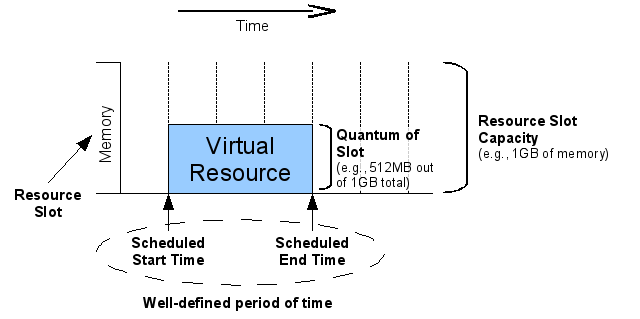
\includegraphics[width=0.8\textwidth]{figures/resourceslot.png}
    \caption{Resource Slot and Virtual Resource}
	\label{fig:resourceslot}
  \end{center}
\end{figure}

In this section, we present a resource management model that enables accurate and efficient creation and management of virtual workspaces in some of the resource management scenarios described in Section~\ref{cha:scenarios}, and which will allow us to tackle the problems described in the previous section. 

Our model assumes a set of physical resources providing a set of \emph{resource slots} (e.g., all the physical memory is one resource slot, each CPU is another resource slot, etc.). A quantum of a slot (e.g., 512 MB of memory, out of the 4 GB available) may be bound to a virtual workspace to provide it with some hardware resources needed to support the workspace's activities for a \emph{well{}-defined period of time}. We term such a binding of a portion of a slot to a virtual workspace a \emph{virtual resource}. All these concepts are summarized in Figure~\ref{fig:resourceslot}

Existing local resource managers, geared towards managing the execution of jobs, are not adequate for scheduling virtual resources because they would not take into account the overhead involved in deploying and managing those virtual resources. In particular, we encounter two types of overhead, which were alluded to in the previous section: \emph{preparation} and \emph{runtime}. The former refers to the cost of preparing the environment where the virtual workspace will run (most notably, deploying the VM images required by that workspace), while the latter refers to the memory, CPU and I/O overhead incurred by the VM hypervisor itself. Furthermore, these overheads are not necessarily constant, and may depend on the size of the requested virtual resources, the hypervisor used, and the quality of base resources.

\begin{figure}
  \begin{center}
(a)

    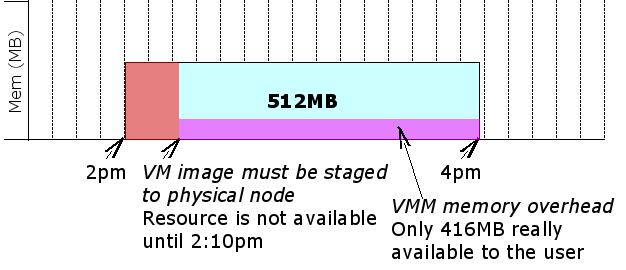
\includegraphics[width=0.8\textwidth]{figures/virtualresources_a.png}

\vspace{3em}
(b)

    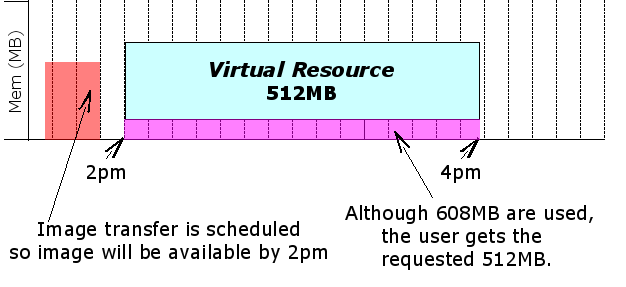
\includegraphics[width=0.8\textwidth]{figures/virtualresources_b.png}



    \caption{Virtual Resources and Overhead: (a) without considering overhead separately, and (b) considering overhead separately}
	\label{fig:virtualresources}
  \end{center}
\end{figure}

For example, let us assume that memory and time (availability) are the only two resources, and that a user requests 512MB of memory from 2pm to 4pm to support the execution of a workspace. Figure~\ref{fig:virtualresources}(a) shows how the resources allocated to the user would be diminished by two types of overhead: the preparation overhead of transferring the (potentially large) workspace's VM image to the physical node where it will run, delaying the start time of the workspace, and the runtime overhead of the virtual machine monitor. 

Using existing local resource managers, even those with AR capabilities, affects the accuracy of virtual workspace deployments, since they burden users with having to factor in the different types of overhead into their resource requests. This task is not easy because users cannot  predict the time to stage the VM image accurately, as they are unaware of the network traffic conditions on the site, and they have no control over how much of the virtual machine monitor's overhead will be deducted from their allocation (e.g., if several VM's are deployed on a single physical node, the deduction might be shared).

Thus, we argue in favor of a \emph{virtual resource management model}, where users get \emph{exactly} the resources they requested. To accomplish this, portions of resource slots can be bound either to virtual resources \emph{or}
to overhead in our model. The virtual resource accurately represents the resources requested by the user, and overhead is managed \emph{separately}, instead of being \emph{deducted} from the user's allocation. This results in more work for the local scheduler, which must now schedule both the virtual resource and the overhead, but results in increased accuracy and, as we will discuss in the following sections, enables the scheduler to take steps towards reducing overhead (increased efficiency).

For example, Figure~\ref{fig:virtualresources}(b) shows how a user's request for 512MB of memory from 2pm to 4pm is processed accurately by (1) \emph{scheduling} the preparation overhead of transferring the VM image (by prestaging it to the physical node before the scheduled start time of the virtual resource) and by (2) setting aside enough memory for the runtime overhead of the virtual machine without deducting it from the virtual resource.

Nonetheless, managing virtual resources and overhead involves challenges along several dimensions:

\begin{description}
\item[Time] (or \emph{availability}: We must guarantee that resources are available at the agreed--upon time, and must be able to reject requests that are deemed infeasible because it would not be possible to set up the required environment on time.
\item[Memory]: We must take into account that part of the memory in a physical node must be assigned to the virtual machine monitor. This dimension is trivial, since this memory usage is generally constant.
\item[Networking]: We must take into account that network bandwidth is shared by all the VMs on a physical node and with preparation overhead (such as image staging). Furthermore, network usage can affect CPU usage in the virtual machine monitor.
\item[Disk]: Similarly to networking, disk I/O is shared by all VMs on a node and can affect CPU usage in the virtual machine monitor. Furthermore, physical nodes must have enough disk space to support the VM images of different workspaces
\item[CPU]: The CPU share required by the virtual machine monitor can vary over time, depending on the resource usage of the VMs it is managing.
\end{description}

As mentioned in the introduction, we concern ourselves here with the resource dimension of availability, which is primarily affected by preparation overhead. In particular, workspace deployment can involve the (potentially expensive) transfer of a VM image to a node, a task that requires I/O and network usage that must be accounted for by the scheduler. However, we currently assume that VMs produce no network activity that would share bandwidth with preparation overhead (i.e. the Networking dimension does not affect the Time dimension).

The management of runtime overhead for the Xen virtual machine monitor was explored previously by Freeman et al. \cite{DBLP:conf/icsoc/FreemanKFRSW06}, and we leave an investigation of multi--dimensional scheduling of both preparation and runtime overhead for future work.



\chapter{Design}
\label{cha:design}
In this section we describe the design of a virtual machine scheduling system that manages virtual resources and preparation overhead separately, using scheduling strategies designed to increase accuracy and efficiency. In particular, we will discuss (1) how our scheduling system allocates resources for Best-effort and AR requests, (2) a set of file staging strategies for VM image deployment, and (3) a strategy for reusing VM images on physical nodes.

\section{Best-Effort and AR scheduling}
\label{sec:scheduling}

Our system supports scheduling of best--effort requests and closed advance reservation requests (described in Section~\ref{cha:scenarios}). For best--effort requests, we currently only support serial requests, where the individual VMs in a workspace do not need to run in parallel (this is similar to serial batch jobs). Advance reservations, on the other hand, always request VMs in parallel: all the VMs in an advance reservation will begin at the same time, and a request will be rejected if there are not enough resources for all the VMs at the same time.

A best--effort request includes the following information:

\begin{itemize}
\item[---] Number of VMs in the request.
\item[---] Resources required by the VM. We currently support specifying the number of CPUs and amount of memory required by each VM.
\item[---] Maximum duration of each VM.
\item[---] VM image required. This is specified by a URI pointing to the image's location in an image repository node.
\end{itemize}

Best--effort requests are scheduled using a FCFS (First Come First Serve) algorithm. As requests arrive, they are placed on a queue. In turn, the head of the queue is inspected every scheduling quantum, and if there are enough resources to run a single VM at that time, the VM is scheduled for deployment and execution. Since the VMs are serial--scheduled, this process does not involve any backfilling or resource reservation strategies, except in the presence of advance reservations (a case which is explained next).

An advance reservation includes the same information as a best--effort request, but also includes a specific start time at which all the VMs in the request must start. The end time of the reservation will be computed as \emph{start time + duration}. To schedule advance reservations, our scheduler models physical resources as resource slots (as described in the previous section) where we must fit a given request for an advance reservation. To perform this slot--fitting, we first determine if the request it feasible at the requested start and end times and, if there is a choice of physical nodes, we greedily choose the nodes that would minimize the number of image transfers. In particular, we do the following:

\begin{itemize}
\item[---] We have a request for $n$ VMs, starting at time $t_s$ and ending at time $t_e$, each requiring $r_i$ resources (for all $i$ types of resources: CPU, memory, etc.). Each physical node has $R_i$ total resources.
\item[---] Find the physical nodes at time $t$ such that the number of available resources $R_i'$ in each node is $\geqslant r_i$ (i.e., we can fit at least one VM on that node). Make sure that those resources are available up until $t_e$. This is our list of candidate nodes
\item[---] Order the list of candidate nodes, giving priority to nodes where we will be able to reuse already deployed VM images (this is described below in Section~\ref{sec:reuse}), and then to nodes where we can deploy more than one VM. 
\item[---] Traverse the list of candidate nodes and, at each node, fit as many VMs as possible. If we manage to fit all the VMs, we know that the VM component of the reservation is feasible.
\item[---] Before completely accepting the reservation, and committing it in the scheduler, we must check that it will be possible to transfer all necessary VM images by $t_s$. This is described below in Section~\ref{sec:filestaging}
\end{itemize}

\begin{figure}
  \begin{center}
    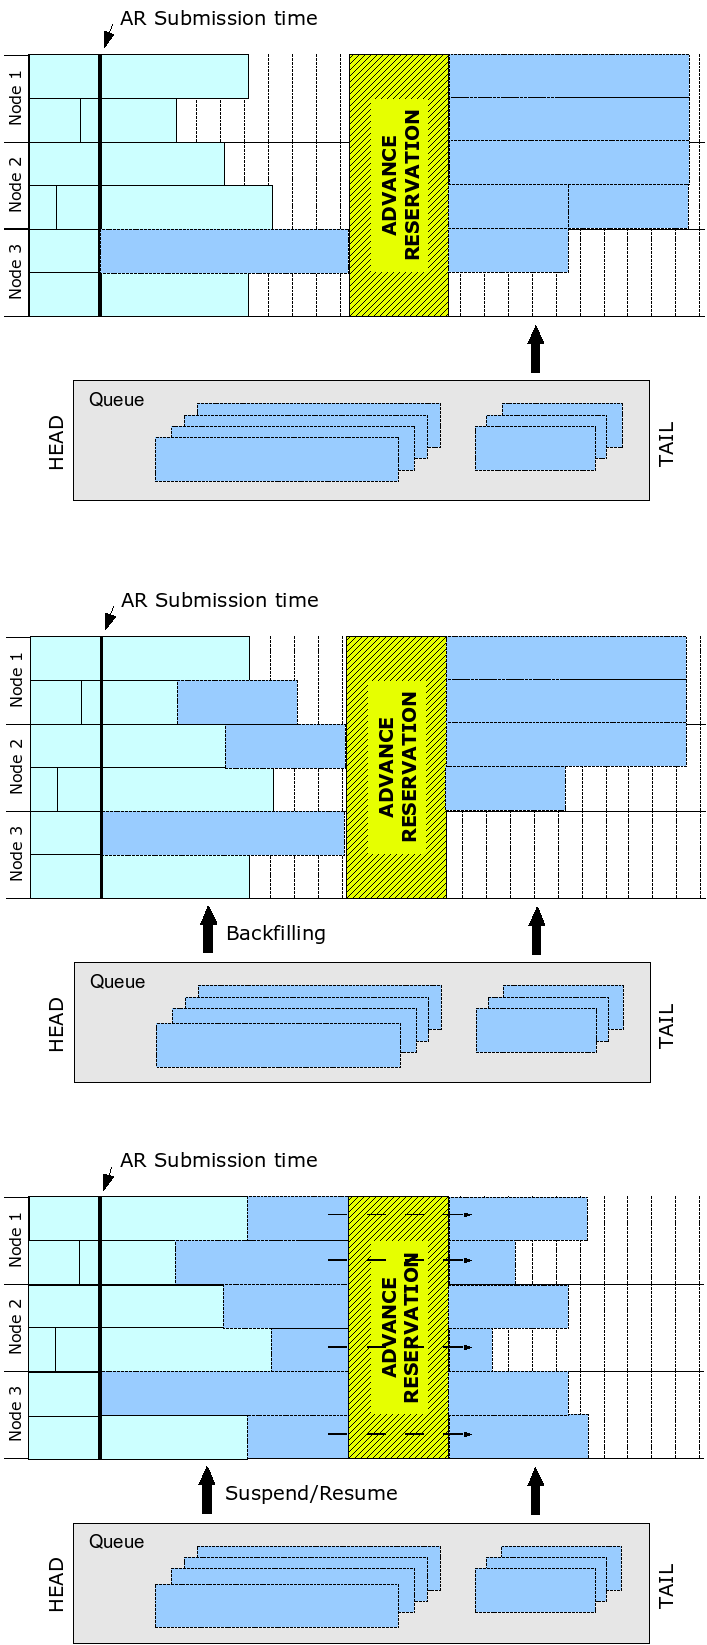
\includegraphics[height=1\textheight]{figures/arbatch.png}
    \caption{Top: Draining nodes before an AR. Middle: Backfilling the time before an AR. Bottom: Suspending before an AR, and resuming after the AR.}
	\label{fig:backfilling}
  \end{center}
\end{figure}


When combining best--effort requests and advance reservations, we can find that the time before an advance reservation is underutilized, as we cannot schedule any best-effort requests that would end after the scheduled start time of the advance reservation (see Figure~\ref{fig:backfilling}, top diagram). This is a common problem in parallel job scheduling, where resources can be allocated for a parallel job (requiring several CPUs in parallel), but the resources before the parallel job might not be able to satisfy the requirements of the next job in the queue. \emph{Backfilling} strategies \cite{10.1109/ICPPW.2002.1039773,feitelson02analyzing,feitelson04parallel} allow lower--priority jobs to run in the time before a parallel job, without affecting the starting times of higher priority jobs (see Figure~\ref{fig:backfilling}, middle diagram).

In a batch scheduler, different backfilling strategies differ on how they reserve resources for parallel jobs in the queue. However, our system does not support parallel best--effort requests (the equivalent of parallel jobs in batch schedulers), and we are only interested in backfilling the time before an advance reservation (which cannot be scheduled on a best--effort basis, like a parallel job) with best-effort serial requests. In this case, the task of backfilling becomes much simpler, and is reduced to traversing the queue in search of VMs which can be scheduled before the advance reservation.

However, as shown in Figure~\ref{fig:backfilling}, backfilling can still result in some underutilization. Another alternative is to suspend best--effort requests before an advance reservation, and resume them as soon as the advance reservation ends (see Figure~\ref{fig:backfilling}, bottom diagram). \emph{Suspend/resume} is not a novel strategy, as many existing resource managers, such as Condor and SGE, allow checkpointing of jobs. However, this feature generally requires modifying a job's executable to support checkpointing, although in some cases this can be achieved by adding checkpointing support to an OS kernel \cite{blcr}. VMs, on the other hand, allow a machine to be suspended/resume seamlessly, without modifying the software that will be running inside the VM.


\section{File staging strategies}
\label{sec:filestaging}

Jobs submitted to batch schedulers generally assume that the required files are available in the worker nodes (e.g., through an NFS drive) or that the input files will be staged to the worker nodes when the job starts. As discussed in the previous section, this assumption presents problems for deploying time{}-sensitive VWs, as VM images can be large and costly to transfer, and transfer times can consume a significant portion of the time allocated to the user. Thus, even if a resource is made available at a requested time $t$, it may not be ready for use until a significantly later time $t+d$.

These problems can be solved in some cases by providing the scheduler with application--specific information about what data needs to be transferred for each deployment, enabling it to distinguish cases where prestaging the data before the scheduled start time $t$ would be appropriate. In the case of a virtual workspace, the application--specific information provided to the scheduler is the workspace metadata file, which contains information the scheduler can use to estimate the amount of preparation overhead (the time necessary to transfer the required VM images). In particular, the relevant information is (1) an image descriptor (currently the location of the image file within an image repository node), (2) the image size, and (3) the number of nodes in the VW.

As described in our virtual resource model, preparation overhead would be managed separately from the virtual resources. Thus, we propose the use of a \emph{scheduled} file transfer strategy: after estimating the amount of preparation overhead, the image transfers are scheduled to complete by time $t$, and the scheduler will reject workspaces where such an image transfer cannot be scheduled (even if all other resources, such as CPU and memory, are available during the requested period of time). In particular, for ARs we schedule image transfers using an Earliest Deadline First (EDF) algorithm \cite{BorjaCite22}. Using EDF allows us to guarantee that image transfers complete by time $t$ (the deadline), while also allowing us to distinguish what image transfers are infeasible. Since EDF is an aggressive algorithm (image transfers begin as soon as possible, even if the deadline is still far away), we also use a just--in--time variation on EDF, which we term EDF/JIT, where image transfer are still sorted according to their deadlines, but pushed as close as possible to the deadline. Figure~\ref{fig:edf} illustrates these two strategies.

\begin{figure}
  \begin{center}
    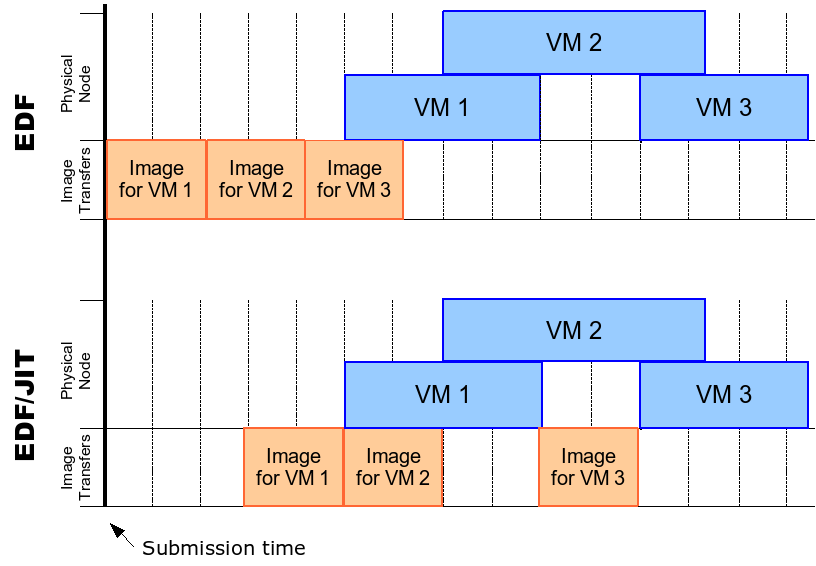
\includegraphics[width=0.8\textwidth]{figures/edf.png}
    \caption{EDF and EDF/JIT file staging strategies}
	\label{fig:edf}
  \end{center}
\end{figure}

Best--effort reservations lack the deadline--sensitive component of AR reservations, so we use a simple FIFO queue to schedule image transfers for these reservations. We currently assume that image transfers for ARs and best--effort reservations are scheduled separately, and we leave the development of an algorithm combining the deadline--sensitive aspect of EDF and the best--effort aspect of FIFO for future work.


\section{Reusing VM images}
\label{sec:reuse}

Adequate VM image staging affects \emph{accuracy}, by making sure that all preparation overhead is processed before the virtual workspace's scheduled start time. We also wish to improve \emph{efficiency} by reducing preparation overhead whenever possible. We accomplish this by reusing VM images already deployed on physical nodes. As described in Section~\ref{sec:vwrepresentation}, factoring deployment--independent configuration information out of the VM image and into a metadata file allows VM images to be reusable. In particular, a VM image can be deployed to a physical machine, and used multiple times by making local copies and binding those copies to potentially different metadata files. This reusability enables us to keep VM image templates on a physical node and using them for several different deployments, thus reducing the number of image transfers.

Our image reuse algorithm requires that each physical node have a certain amount of disk space reserved for an \emph{image pool}. This pool will contain image templates, not bound to any workspace metadata, which can be shared by different deployments. Assuming an empty pool on a node, the deployment of a VW on that node would result in the following steps:

\begin{enumerate}
\item Since the pool is empty, deploying this VW will require transferring an image to that node.
\item Once the transfer is completed, the image is added to the pool, and assigned a \emph{timeout}. This timeout will initially match the end time of the VW, to guarantee that it will remain in the pool for, at least, the duration of the VW.
\item Since we do not want to modify the image (so it can be potentially reused by other VWs), the VW does not use the image in the pool directly. Instead, if the system supports it, it will access the image using \emph{copy--on--write} (COW). If COW is not supported, a local copy of the image will be made before the VW starts.
\item When the timeout of the image is reached, the image is removed from the pool.
\end{enumerate}

Reuse of images is, essentially, accomplished by extending the timeout of the images in the pool to accommodate future deployments. So, let's assume that an image $A$ is deployed, with timeout $t_\textrm{expire}$, on node $N1$, to be used by VW \#1. At some point, a request arrives for VW \#2 starting at time $t_\textrm{start}$ and ending at time $t_\textrm{end}$. If $t_\textrm{start} \leqslant t_\textrm{expire}$ (i.e., the image is guaranteed to be in the image pool at time $t_\textrm{start}$), we flag that image $A$ will also be used by VW \#2, and the timeout will be updated to $t_\textrm{end}$. When $t_\textrm{start}$ arrives, VW \#2 will reuse image $A$ as described above: by using COW or making a local copy.

When scheduling VWs, the scheduler will take into account the state of the image pools in each node, and will attempt to minimize the number of image transfers by allocating, whenever possible, VWs to nodes where the required image is already a part of the image pool. This algorithm also has allows administrators to set a limit on the size of the image pool, making sure that disk usage by VM images will not grow without bounds. The tradeoff, of course, is that some VWs might be rejected since the required VM image is not available in the image pool and cannot be transferred because it would make the image pool too big.

Finally, it should be noted that the strategy of reusing images benefits both AR deployments, since it will be possible to accept starting times that would ordinarily be unfeasible if the image first had to be transferred to the nodes, and best--effort deployments, by allowing workspaces to start running sooner.

\subsection{Avoiding redundant transfers}

\begin{figure}
  \begin{center}
    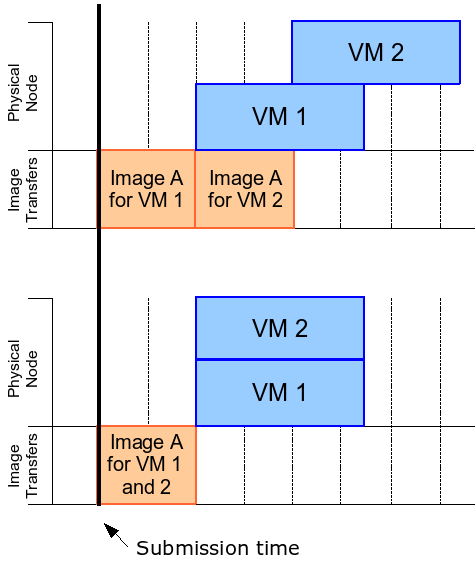
\includegraphics[width=0.6\textwidth]{figures/piggybacking.png}
    \caption{Avoiding redundant transfers}
	\label{fig:piggyback}
  \end{center}
\end{figure}

As an additional optimization to our image reuse algorithm, image transfers are also scheduled in such a way that redundant transfers are avoided. There are two types of redundant transfers we wish to avoid:

\begin{description}
\item[Transfers for ARs:] Assume that a transfer for image $A$ has been scheduled to arrive on node $N1$ at time $t_{1,\textrm{start}}$. This image will be used by VW \#1 (ending at $t_{1,\textrm{end}}$). At some point before $t_\textrm{start}$, a request for VW \#2 arrives, also requiring image $A$, starting at $t_{2,\textrm{start}}$ (where $t_{2,\textrm{start}}>t_{1,\textrm{end}}$) and ending at time $t_{2,\textrm{end}}$. The scheduler determines that VW \#2 should be assigned to node $N1$. Scheduling an additional transfer would be redundant, since there is already a transfer for $A$ scheduled for that node. So, the existing transfer is tagged as carrying an image to be shared by VM \#1 and VM \#2. One the transfer is completed, the image's timeout in the pool will be $t_{2,\textrm{start}}$ (or, more generally, $\textrm{max}(t_{1,\textrm{end}},t_{2,\textrm{end}})$)
\item[Transfers for best--effort reservations:] As shown in Figure~\ref{fig:piggyback} (top), assume that the last image transfer scheduled on the FIFO queue for best--effort reservations carries image $A$ to node $N1$, set to arrive at time $t_\textrm{start}$ to be used by VM \#1. Also, assume that the time to transfer image A is $t_A$. Now, a request for a new best--effort reservation arrives for VM \#2, also requiring image $A$. If we scheduled a separate image transfer for VM \#2, it would start at $t_\textrm{start}+t_A$, despite the availability of resources at $t_\textrm{start}$. By allowing the transfer to piggyback on the previously scheduled transfer, VM \#2 can start earlier, as show in Figure~\ref{fig:piggyback} (bottom)
\end{description}

To avoid these redundant transfers, the scheduler will inspect the image transfer schedule when processing a new request to ascertain if existing image transfers can be reused. In particular:

\begin{description}
\item[Transfers for ARs:] Given a VW starting at time $t_\textrm{start}$ and ending at time $t_\textrm{end}$, requiring image $I$, assigned to node $N$. If there is an image transfer of $I$ scheduled to $N$, with deadline less than or equal to $t_\textrm{start}$, then simply reuse that transfer. Furthermore, the scheduler will take into account existing transfers when mapping requests to nodes (assuming availability of resources in the nodes, it is preferable to schedule a VW to a node with a reusable image transfer than scheduling it to a node where a new image transfer would necessarily have to be scheduled).
\item[Transfers for best--effort:] Given a VW requiring image $I$, the scheduler checks not only the state of the image pools, but also the upcoming transfers in the FIFO transfer queue. This way, it may be possible to schedule a best--effort VW sooner by reusing an existing transfer than by adding an additional transfer to the FIFO queue.
\end{description}







\chapter{Implementation}
\label{cha:impl}
We produced two implementations for our experiments:

\begin{description}
\item[SGE--based:] We add a layer of scripts on top of an existing local resource manager, Sun Grid Engine
\cite{sgeweb}, or SGE. These scripts take the application--specific information of virtual workspaces (the metadata file), and use SGE to schedule not only the virtual resources, but also the preparation overhead. We chose SGE precisely because it is easily extensible, and we could add some of our extensions without having to modify the SGE source code itself.

However, this is only a partial implementation of the techniques described in the previous section, since SGE does not support advance reservations or suspend/resume. In effect, we are limited to testing best--effort workloads. We can also experiment with AR workloads, but only to the point of finding a schedule for a set of image transfers which is already known to be feasible (since SGE cannot perform this kind of admission control). Furthermore, image reuse is accomplished through the use of a simple LFU cache, instead of the reuse algorithm described in the previous section.

Nonetheless, this implementation is allows us to test our image prestaging and reuse techniques on physical hardware.
\item[Simulator:] A scheduler developed by us which implements all the tecniques described in the previous section. Currently, this scheduler does not interact with a real testbed and runs in simulation. 

The scheduler, and simulated backend, are implemented in Python. The scheduling information is stored in a relational database, implemented with SQLite. 
\end{description}


\chapter{Experiments}
\label{cha:experiments}
We present a series of experiments that illustrate the effect of using
the scheduling model and techniques discussed in the previous section.
These experiments focus on evaluating our techniques for managing the
overhead of transferring VM images to the nodes where they are
deployed.

Our experiments are divided into three sets:

\begin{description}
\item[\#1 Accuracy of AR deployments:] Investigates effect of scheduling image transfers on accuracy, using AR--only deployments. These experiments were run on our physical testbed, with our SGE--based implementation. We also ran a simulated experiment to compare disk usage between the EDF and EDF/JIT image transfer algorithms.
\item[\#2 Efficiency in Best--effort deployments:] Investigates effect of image reuse in Best--effort deployments. These experiments were run on our physical testbed, with our SGE--based implementation.
\item[\#3 Mixing Best--effort and AR workloads:] Investigates what types of mixed workloads (Best--effort and AR) stand to benefit from using VMs, by using all of the techniques discussed in the previous sections. We focus on measuring the effect that virtualization has on utilization and running time of mixed workloads. These experiments were run using our simulator.
\end{description}

The physical testbed for experiments \#1 and \#2 is composed of 10 dual{}-CPU Pentium
III 500 MHz systems, each with 512 MB of RAM and 9G of local disk. One
node was used as a cluster head node, eight nodes for VM deployment,
and the remaining node as an image repository node, from which the VM
images would be transferred to the worker nodes. Nodes were connected
using 100 Mb/s switched Ethernet.

Virtual machine images were deployed using the SGE scheduler with the
extensions described in the previous section, based on traces that we developed for both
the advance reservation (AR) and best--effort cases. For the best--effort
cases, we used real workload traces, while for the AR cases, lacking
real AR submission workloads, we produced artificial traces using a
trace generator.

The simulated testbed used for part of experiment \#1 and for experiment \#3 is also composed of 10 dual{}--CPU nodes, each with 1GB of memory, with eight worker nodes, one head node, and an image repository node. Nodes are connected using a 100 Mb/s switched Ethernet. We do not impose a limit on the local disk in each node, but keep track of how much disk space is used throughout the experiments. The simulations were run on the University of Chicago's Department of Computer Science's Condor pool.

For all our experiments, we assumed that all virtual workspace requests
involved the same amount of CPU\% and memory for each virtual node. We
allowed at most 2 VMs to be deployed to a single physical node. Since
we focus on preparation overhead, the VW remains idle during its
runtime. As described in Section~\ref{cha:virtualresources}, we assume that the VM generates no network traffic that
would share bandwidth with preparation overhead. 

%The results from Experiments \#1 and \#2 (except the disk usage results from experiment \#1) were first presented in Sotomayor et al. \cite{overheadmatters}.

\section{Accuracy of AR deployments}

% Clarify that we are not using caching here.

Our first set of experiments investigates to what extent using
information on the relatively manageable overhead of VM scheduling can
improve the accuracy of providing a virtual resource to a
deadline{}-sensitive client. We assume that the client requests an advance reservation and we calculate accuracy (or
``client satisfaction'') as the ratio of the time the client actually
got to the requested time. Lacking any AR traces or existing AR trace generators,
we developed a simple trace generator capable of generating a large
number of requests according to a set of parameters. Since our SGE--based implementation does not support advance reservations, we then ran an
offline admission control algorithm on those requests to ensure that there exists a feasible
schedule for the submissions in the trace. Each submission represents
the deployment of a virtual cluster configured with the software
required to applications commonly run on the Open Science Grid (OSG),
and includes (1) the descriptor of the image template to use, (2) the
number of nodes, (3) the starting time of the workspace, and (4) its
duration. The Xen VM image with OSG worker node support that we used in
this experiment is 600 MB in size \cite{DBLP:conf/ccgrid/FosterFKSSZ06}. Nonetheless, we do not use any image reuse strategies in this experiment, as goal is to show that scheduling image transfers is, by itself, advantageous.

In this experiments we compare the EDF scheduling algorithm described in Section~\ref{sec:reuse} with non--scheduled file staging strategies. These strategies do not attempt to fit the image transfer in an optimal or near--optimal place in a schedule, but rather base the time of the image transfer directly on a fixed event, such as the submission time of a request or its starting time. The purpose of comparing against these strategies is to show that a scheduled approach not only guarantees accuracy, but it also better than easier--to--implement na\"ive strategies. In particular, we compare against the following (Figure~\ref{fig:filetransfer} summarizes these file staging strategies):

\begin{description}
\item[Job--style:] The image transfer begins at the same time as the start time for the virtual resources.
\item[Just In Time (JIT):] Assuming the network's full bandwidth is available for staging the necessary VM image for a workspace, the scheduler estimates the time required to transfer the image and starts the transfer before the start time, allocating just enough time to transfer the image.
\item[Aggressive:] This strategy attempts to transfer images immediately after the request has been accepted, regardless of the
starting time for the request.
\end{description}

To measure only the effect of image transfer scheduling on accuracy, VM images are not reused on the physical nodes.

\begin{figure}
  \begin{center}
    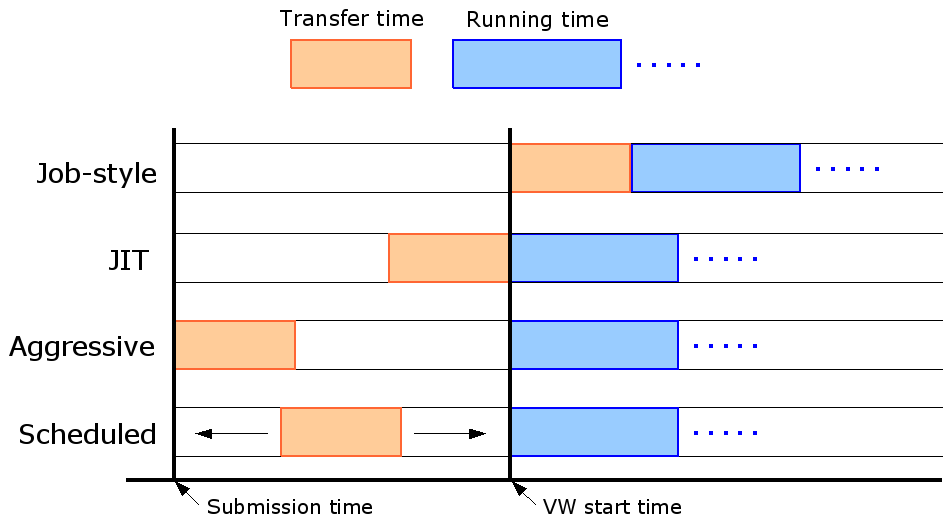
\includegraphics[width=0.8\textwidth]{figures/filetransfer.png}
    \caption{Naïve file staging strategies}
	\label{fig:filetransfer}
  \end{center}
\end{figure}


\newcolumntype{M}{>{\centering}m{0.15\textwidth}}
\newcolumntype{N}{>{\centering}m{0.3\textwidth}}

\begin{table}
\begin{center}
\caption{Traces used in experiments}
\begin{tabular}{|M|MM|MM|}

\cline{2-5}
\multicolumn{1}{M|}{}&
\multicolumn{1}{M|}{\bfseries Trace I}&
\multicolumn{1}{M|}{\bfseries Trace II}&
\multicolumn{1}{M|}{\bfseries Trace III}&
\multicolumn{1}{M|}{\bfseries Trace IV}

\\\hline

{\bfseries Trace duration (s)} &
\multicolumn{2}{N|}{7200}&
\multicolumn{2}{N|}{4700}

\\\hline

{\centering\bfseries \#~VW \nohyphens{submissions}} &
\multicolumn{1}{M|}{36}&
35 &
\multicolumn{2}{N|}{62}

\\\hline

{\bfseries Nodes per VW} &
\multicolumn{2}{N|}{2{}-4\newline (Uniformly distributed)} &
\multicolumn{2}{N|}{2{}-16\newline (Derived from original trace)}

\\\hline

{\bfseries Total images to deploy} &
\multicolumn{1}{M|}{110 (66.0GB)} &
{106\newline (63.6GB) } &
\multicolumn{2}{N|}{114 (86.4GB)}

\\\hline

{\bfseries VW Duration} &
\multicolumn{2}{N|}{1800s} &
\multicolumn{2}{N|}{Avg=53.0s\newline StDev=4.24s}

\\\hline

{\bfseries Starting times} &
\multicolumn{1}{M|}{Uniformly Distributed} &
{Clustered in 100s windows every 900s} &
\multicolumn{2}{N|}{\centering ASAP}

\\\hline

{\bfseries Images used} &
\multicolumn{2}{N|}{6 600MB images,\newline uniformly distributed} &
\multicolumn{2}{N|}{See Table 2}

\\\hline
\end{tabular}
\label{tab:traces}
\end{center}
\end{table}

Table~\ref{tab:traces} describes the two traces (I and II) used in this experiment.
These two traces differ in how the starting times of the VWs are
distributed throughout the duration of the experiment. In Trace I, the
starting times are distributed uniformly throughout the trace, while in
Trace II the starting times appear only during 100s windows (each
occurring every 900s), simulating VWs that are submitted in a bursty
fashion.

\begin{figure}
  \begin{center}
    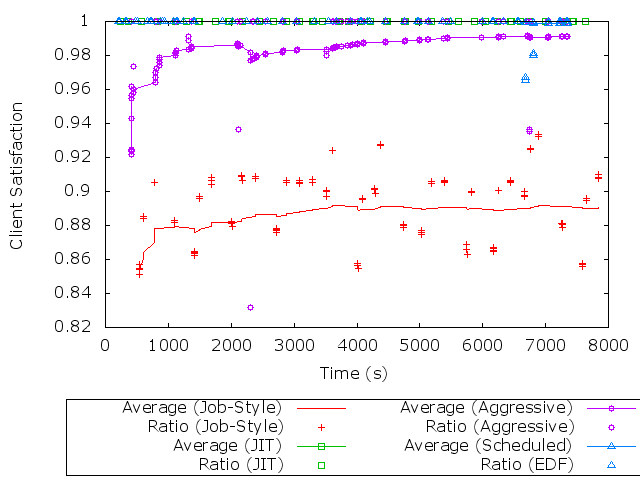
\includegraphics[width=0.8\textwidth]{figures/ClientSatisfaction-UniformStartTimes.png}
    \caption{Client Satisfaction (Trace I)}
	\label{fig:clientsatisfactionI}
  \end{center}
\end{figure}

Figure~\ref{fig:clientsatisfactionI} shows the results of running Trace I with the different image scheduling
strategies. We see that \emph{EDF} and \emph{JIT} achieve 100\%
client satisfaction in most cases, followed by \emph{Aggressive} with
most submissions in the 96\%{}-100\% range. Since this trace represents
a best{}-case scenario, where the start times are uniformly distributed
throughout the experiment, even the na\"ive \emph{JIT} and
\emph{Aggressive} strategies achieve good performance.

\begin{figure}
  \begin{center}
    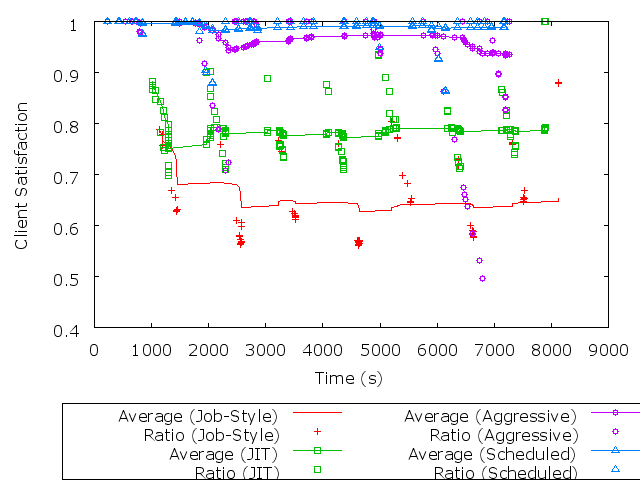
\includegraphics[width=0.8\textwidth]{figures/ClientSatisfaction-ClusteredStartTimes.png}
    \caption{Client Satisfaction (Trace II)}
	\label{fig:clientsatisfactionII}
  \end{center}
\end{figure}

Figure~\ref{fig:clientsatisfactionII} shows results with Trace II. Since \emph{JIT} allows just
enough time to transfer the image, regardless of what other VWs are
scheduled, this strategy can result in multiple image transfers being
scheduled during the same period of time (right before the ``window'').
As those transfers share available bandwidth, they take longer than
estimated. \emph{EDF} addressed this problem by assigning priorities to image
transfers and making use of network idle time, resulting in the best
performance, with few non{}-100\% satisfaction instances (and always at
the end of a ``window''). \emph{Aggressive}, on average, also has
good performance, but the images with tighter deadlines suffer as the
result of having to share bandwidth with other transfers.

\emph{EDF} is the only approach that schedules a resource slot for the preparation overhead with
the goal of maximizing client satisfaction, while the other strategies
na\"ively start the image transfers at fixed times. By scheduling
overhead in the same way as virtual resources, instead of assuming that
overhead should be absorbed into the client's requested virtual
resource, \emph{Scheduled} achieves the best client satisfaction in the
two submission patterns present in traces I and II.

However, due to the limited disk space in our physical testbed, this setup is inadequate to observe how well disk usage scales. To do this, we use our simulator, running a trace of AR requests with the following characteristics:

\begin{itemize}
\item All ARs are known at the beginning of the trace.
\item Number of nodes per AR: 1--16 (uniformly distributed)
\item Number of requests: 94
\item Starting times: Uniformly distributed
\item Duration of trace: 10h
\end{itemize}

We compare the EDF and EDF/JIT image staging algorithms, and measure the peak disk usage in each node at each point in the experiment. Figure~\ref{fig:edfdiskusage} shows how EDF results in a high disk usage at the beginning of the experiment (as high as 31.2GB), since this algorithm will aggressively stage all the images to all the nodes as soon as possible. EDF/JIT, on the other hand, spreads the images transfers throughout the experiment, pushing the transfers as close as possible to the starting times of the reservations. This way, disk usage on any given node never exceeds 2.4GB (four images).

\begin{figure}
  \begin{center}
    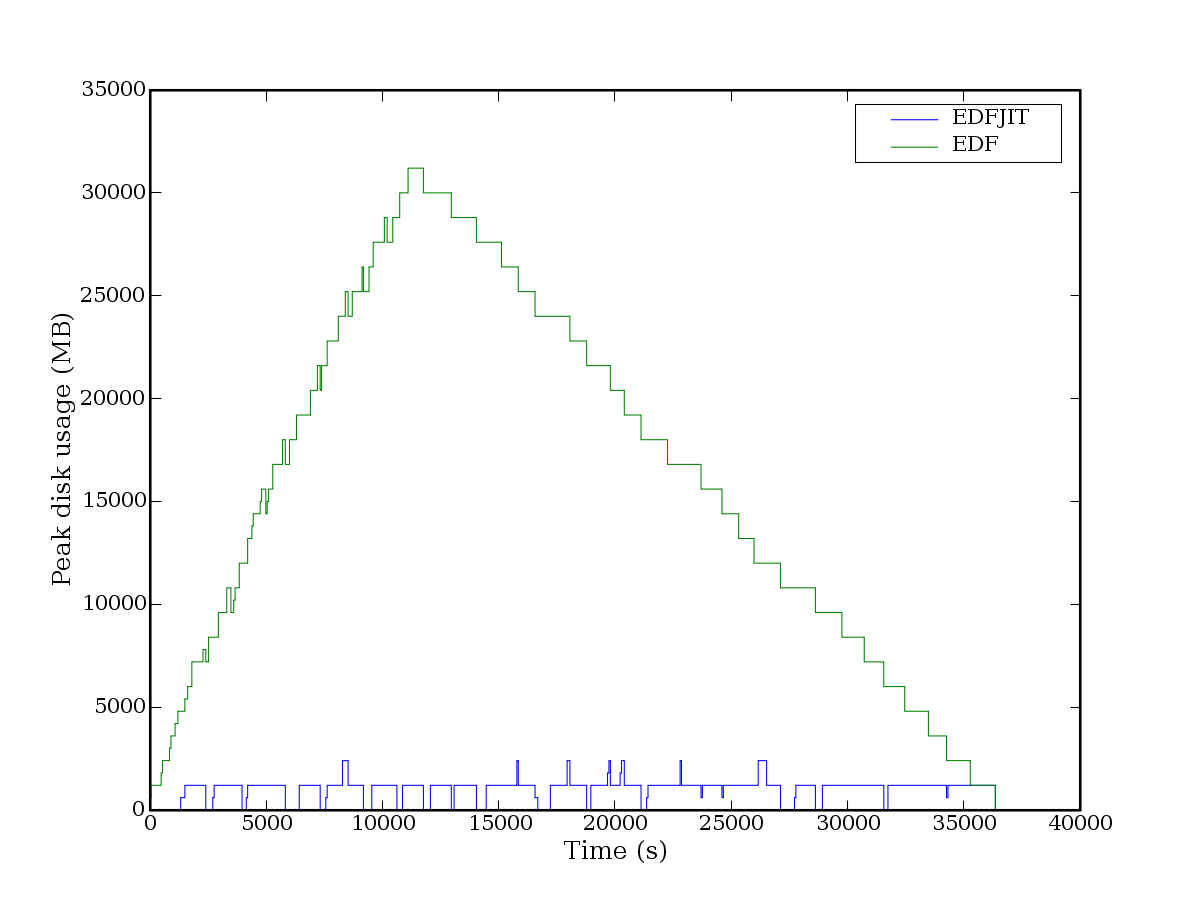
\includegraphics[width=0.8\textwidth]{figures/ar_edf.png}
    \caption{Disk usage with EDF and EDF/JIT}
	\label{fig:edfdiskusage}
  \end{center}
\end{figure}

\section{Efficiency in Best--effort deployments}

Our second set of experiments investigate two things: (1) how much bandwidth the resource provider can save through
judicious use of image reuse based on workspace metadata and (2) to
what extent can image reuse improve deployment time (and thus also
client satisfaction) in situations where VM availability is requested
to start as soon as possible.

Since this experiment focuses on best--effort submissions, the same type of
submissions commonly found in batch systems, we were able to use a real
workload. In particular, we used the San Diego Supercomputer Center
(SDSC) DataStar log, available at the Parallel Workloads Archive \cite{BorjaCite21}.
We chose this workload because it explicitly distinguishes submissions
for the DataStar's express queue (eight 8{}-CPU nodes, accepting jobs
lasting at most 2 hr), which allows us to test a scenario in which
minimizing deployment overhead is specially important: short{}-lasting
jobs. Since the SDSC DataStar log spans several months, we selected an
80 minute stretch of submissions (submissions \#21543 to \#21665 on
queue \#1) for our experiments. We selected this section
because it represents a flurry of short{}-lasting jobs, which
allows us to test how our system copes with the bandwidth requirements
of deploying a large amount of VM images.


\begin{table}
\begin{center}
\caption{Distribution of images in traces III, IV}
\begin{tabular}{|c|c|c|c|c|}
\cline{2-5}
\multicolumn{1}{c|}{} &
\multicolumn{2}{c|}{\bfseries Trace III} &
\multicolumn{2}{c|}{\bfseries Trace IV}

\\\cline{2-5}

\multicolumn{1}{c|}{}  & {\bfseries Submissions} & {\bfseries Images} & {\bfseries Submissions} & {\bfseries Images} 

\\\hline

{\bfseries img.1} & 23\% & 21\% & 55\% & 60\%

\\\hline

{\bfseries img.2}
&
18\%
&
15\%
&
27\%
&
25\%

\\\hline

{\bfseries img.3}

&
15\%
&
12\%
&
6\%
&
6\%

\\\hline

{\bfseries img.4}
&
18\% 
&
15\%
&
5\%
&
4\%

\\\hline

{\bfseries img.5}
&
24\%
&
14\%
&
3\%
&
3\%

\\\hline

{\bfseries img.6}
&
3\%
&
12\%
&
3\%
&
3\%

\\\hline
\end{tabular}
\label{tab:imagedistro}
\end{center}
\end{table}

When adapting the trace to our own experiments, each submission was
converted to a virtual cluster submission in which the number of nodes
was the number of requested processors in the original trace, scaled
down by four (the express queue has 64 processors; our testbed has 16),
with submission times and VW duration left unaltered. Each submission
was assigned one of six 600 MB images. We produced two traces,
with the only difference being the distribution of images assigned to
each submission. The first trace (Trace III) has images uniformly
distributed amongst the submissions, while in the second trace (Trace
IV) two images account for more than 80\% of the submissions. The
characteristics of theses traces are summarized in Table 1, while the
distribution of images is shown in Table~\ref{tab:imagedistro}. The rate at which VWs are
submitted is shown in Figure~\ref{fig:providershape}.

\begin{figure}
  \begin{center}
    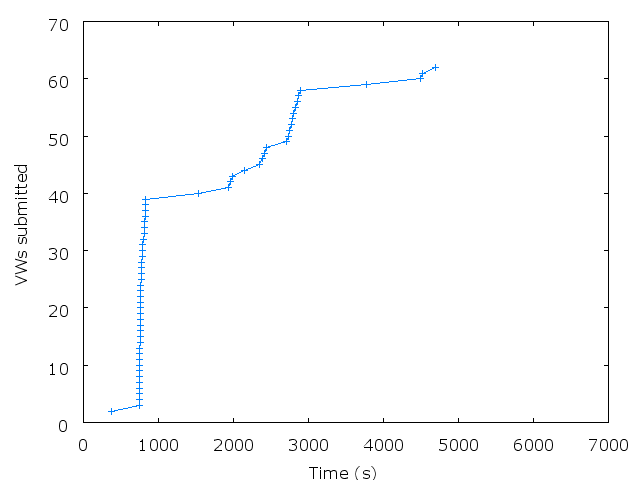
\includegraphics[width=0.8\textwidth]{figures/ProviderPerspective-TraceShape.png}
    \caption{VW Submissions (Traces III and IV)}
	\label{fig:providershape}
  \end{center}
\end{figure}

\begin{figure}
  \begin{center}
    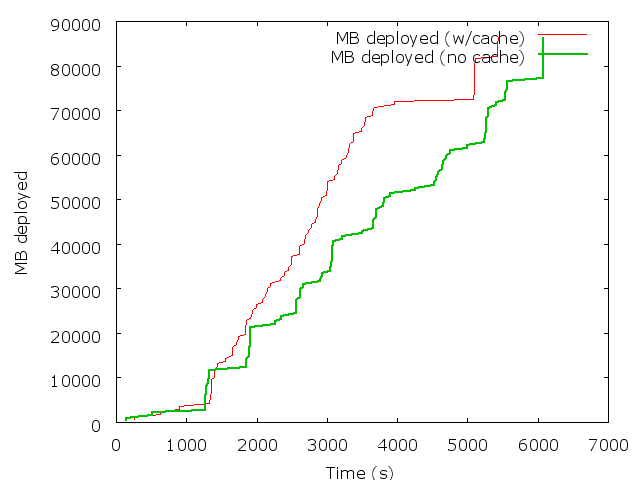
\includegraphics[width=0.8\textwidth]{figures/ProviderPerspective-Uniform2.png}
    \caption{MB Deployed (Trace III)}
	\label{fig:providerIII}
  \end{center}
\end{figure}

\begin{figure}
  \begin{center}
    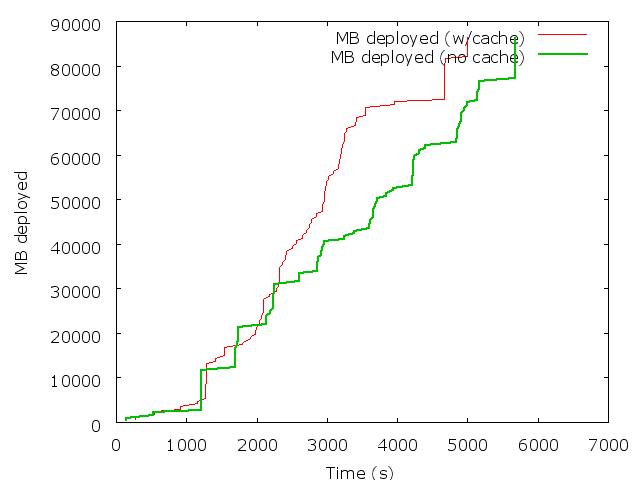
\includegraphics[width=0.8\textwidth]{figures/ProviderPerspective-Pareto2.png}
    \caption{MB Deployed (Trace IV)}
	\label{fig:providerIV}
  \end{center}
\end{figure}

Since these experiments use our SGE--based implementation, we used a 1.8 GB
LFU cache in each node (enough to cache three images) to minimize deployment time and increase throughput.

Figure~\ref{fig:providerIII} shows the cumulative number of MB deployed throughout the experiment. This number reflects how fast images are deployed, whether by an image transfer or reusing an image already cached. So, at a given time, higher values in the graph are better (i.e., more images have been deployed at that time). At any given number of MB (y axis), left--most values are better (i.e., that number of MB has been deployed earlier). We can observe how, after the 2000s mark, the rate at
which images are deployed starts to increase, thanks to the reduced
transfer time resulting from the use of a cache. The difference in
effectively deployed MB is greatest at the 3550s mark, where the cached
approach results in a 25.2 GB ``advantage'' over the non{}-cached
approach. Figure~\ref{fig:providerIV}, shows the same data from running trace IV, where
the distribution of images favors a much larger number of cache hits.
Throughput is slightly better, with a difference of 27.6 GB at that
same 3550s mark.

Deployment time, or the time between when deployment starts and the VMs are ready to run, is also improved. The average
deployment time for a single image, when not using a cache, is 440s for
both traces. This time is reduced to 305s and 247s, in Trace III and IV
respectively, when using an image cache.

These two experiments highlight how using the VW metadata to reuse image
templates and avoid redundant transfers benefits both the provider, by
offering a better utilization of resources leading to higher
throughput, and the consumer, by reducing the deployment time of best--effort
workspaces.


\section{Mixing Best--effort and AR workloads}

Our third set of experiments measures the effect of using our virtual resource model on workloads that combine both AR and best--effort requests. In these experiments, we are interested in observing the time to complete all best--effort requests and the utilization of physical resources.

We use several artificially--generated traces that mix best--effort requests and advance reservations. These traces request enough resources such that, even with 100\% utilization throughout the experiment, each would require between 10h and 10.5h to complete. All ARs are known in advance by the scheduler (i.e., the requests are processed at the beginning of the trace), with starting times uniformly distributed throughout the experiment time. Best--effort requests arrive throughout the duration of the experiment, separated by uniformly separated intervals. 

We generate 36 different traces where we vary three parameters:

\begin{description}
\item[Proportion of Best--effort/AR requests:] This proportion is measured in terms of total running time requested by each type of request if they were run in sequence. For example, a workload with 10 advance reservations, each requesting two virtual nodes with a duration each of 5 minutes (total duration = $10\cdot 2\cdot 5$ = 100 minutes), and five best--effort requests, each requiring 10 virtual nodes with a duration each of 12 minutes (total duration = $5\cdot 10\cdot 12$ = 300 minutes), would be a proportion of 25\% AR and 75\% Best--effort. 

The purpose of this parameter is to observe the effect an increasing number of ARs can have on a Best--effort workload. We use the following proportions:
\begin{itemize}
\item 25\% Best--effort, 75\% AR
\item 50\% Best--effort, 50\% AR
\item 75\% Best--effort, 25\% AR
\end{itemize}
\item[Duration of best--effort requests:] A best--effort request will require $n$ virtual nodes, each running for time $t$, and scheduled serially (i.e., the nodes do not have to run in parallel). We explore different durations, to explore the effect on the backfilling and suspend/resume strategies (as described in Section~\ref{cha:design}, backfilling will be less effective in the presence of long--duration requests). We use the following durations:
\begin{itemize}
\item short: Average duration = 5 minutes
\item medium: Average duration = 10 minutes
\item long: Average duration = 15 minutes
\end{itemize}
It should be noted that, since we want the total duration of the workload to be ~10h, the value of $n$ will be inversely proportional to $t$. For example, if we reduce the duration of the best--effort requests, we must also increase the number of such requests. The actual value of $n$ will be determined by the proportion of Best--effort and AR requests. So, this parameter also allows us to observe what happens when the total number of best--effort requests in a trace increases (which will involve a larger number of image transfers).
\item[AR resource consumption:] This parameter controls how many physical resources are consumed by an AR request. This translates to how many virtual nodes are requested by an AR (a minimum of 1 and a maximum of 16, in our simulated testbed with 8 physical nodes, each with a capacity for 2 VMs). We explore the following values:
\begin{itemize}
\item Up to 25\% of available physical resources (1--4 nodes)
\item 25\% to 50\% (5--8 nodes)
\item 50\% to 75\% (9--12 nodes)
\item 75\% to 100\% (13--16 nodes)
\end{itemize}
\end{description}

We currently choose one value from each parameter (e.g., choosing parameter \emph{short} results in all best--effort requests having a short duration). This will allow us to observe the behaviour of our scheduler in the limits of these parameters, and we leave more elaborate combinations of parameters (e.g.,traces with 25\% short requests, 25\% medium requests, and 50\% long requests) for future work.

Each request in a trace is assigned a VM image out of 37 possible 600MB images (22.2GB total). The distribution is skewed in such a way that seven images account for 70\% of requests (10\% each), and the remaining images account for 30\% of requests (1\% each). Since disk usage is one of our concerns, this distribution of images allows us to verify that our file prefetching and reusage strategies avoid accumulating all 37 images on the nodes. Furthermore, this case is an example of when predeployment of all the images might not be an acceptable solution (e.g., if we were dealing with 5GB images, that would mean using 185GB on each physical node), 

\subsection{Performance with predeployed VM images}

We start by running the traces in the following two configurations:

\begin{description}
\item[No virtualization] The time before an AR is backfilled (as described in Section~\ref{cha:design}), and there are no images to deploy.
\item[Virtualization, with predeployed images] Before an AR, best--effort requests are suspended and resumed after the AR (as described in Section~\ref{cha:design}, there are no images to deploy, and we assume a 10\% runtime overhead.
\end{description}

The purpose of comparing these two configurations is to observe what types of traces benefit the most from using the suspend/resume capabilities of virtual machines, despite the presence of runtime overhead, and under the assumption that image predeployment is acceptable. Table~\ref{tab:noVMvsPredeploy} shows time (in seconds) required to complete all the best--effort requests. Values in italics denote a case where using VMs results in better performance (shorter running time).

\begin{table}
\begin{center}
\caption{Effect of virtualization (assuming predeployed images) on time to complete best--effort requests}
\textbf{(1)} No virtualization (time in seconds)
\textbf{(2)} Virtualization, with predeployed images (time in seconds)
\begin{tabular}{|c|c|c|c|c|c|}
\hline
\textbf{Duration} & \textbf{AR resources} & \textbf{Batch-AR} & \textbf{(1)} & \textbf{(2)}& \textbf{$\frac{(2)}{(1)}$}
\\\hline
long & 000-025 & 25-75 & 38880 & 39000 & 0.309\%
\\\hline
long & 000-025 & 50-50 & 41160 & 41880 & 1.749\%
\\\hline
long & 000-025 & 75-25 & 41160 & 43500 & 5.685\%
\\\hline
long & 025-050 & 25-75 & 38400 & 37200 & \textcolor{blue}{\textit{-3.125}\%}
\\\hline
long & 025-050 & 50-50 & 41820 & 39360 & \textcolor{blue}{\textit{-5.882}\%}
\\\hline
long & 025-050 & 75-25 & 41100 & 42360 & 3.066\%
\\\hline
long & 050-075 & 25-75 & 37260 & 37020 & \textcolor{blue}{\textit{-0.644}\%}
\\\hline
long & 050-075 & 50-50 & 37320 & 37500 & 0.482\%
\\\hline
long & 050-075 & 75-25 & 42060 & 40080 & \textcolor{blue}{\textit{-4.708}\%}
\\\hline
long & 075-100 & 25-75 & 38700 & 37020 & \textcolor{blue}{\textit{-4.341}\%}
\\\hline
long & 075-100 & 50-50 & 41160 & 37260 & \textcolor{blue}{\textit{-9.475}\%}
\\\hline
long & 075-100 & 75-25 & 45780 & 42180 & \textcolor{blue}{\textit{-7.864}\%}
\\\hline
medium & 000-025 & 25-75 & 38700 & 39060 & 0.930\%
\\\hline
medium & 000-025 & 50-50 & 40800 & 42900 & 5.147\%
\\\hline
medium & 000-025 & 75-25 & 40140 & 43140 & 7.474\%
\\\hline
medium & 025-050 & 25-75 & 36840 & 36960 & 0.326\%
\\\hline
medium & 025-050 & 50-50 & 37200 & 37020 & \textcolor{blue}{\textit{-0.484}\%}
\\\hline
medium & 025-050 & 75-25 & 41220 & 42780 & 3.785\%
\\\hline
medium & 050-075 & 25-75 & 33420 & 33780 & 1.077\%
\\\hline
medium & 050-075 & 50-50 & 37260 & 36780 & \textcolor{blue}{\textit{-1.288}\%}
\\\hline
medium & 050-075 & 75-25 & 40800 & 41520 & 1.765\%
\\\hline
medium & 075-100 & 25-75 & 37380 & 36600 & \textcolor{blue}{\textit{-2.087}\%}
\\\hline
medium & 075-100 & 50-50 & 38640 & 37860 & \textcolor{blue}{\textit{-2.019}\%}
\\\hline
medium & 075-100 & 75-25 & 40800 & 40860 & 0.147\%
\\\hline
short & 000-025 & 25-75 & 36120 & 38700 & 7.143\%
\\\hline
short & 000-025 & 50-50 & 40860 & 43260 & 5.874\%
\\\hline
short & 000-025 & 75-25 & 41820 & 45240 & 8.178\%
\\\hline
short & 025-050 & 25-75 & 36600 & 36540 & \textcolor{blue}{\textit{-0.164}\%}
\\\hline
short & 025-050 & 50-50 & 40380 & 41340 & 2.377\%
\\\hline
short & 025-050 & 75-25 & 41160 & 43140 & 4.810\%
\\\hline
short & 050-075 & 25-75 & 30960 & 31020 & 0.194\%
\\\hline
short & 050-075 & 50-50 & 36900 & 37200 & 0.813\%
\\\hline
short & 050-075 & 75-25 & 39180 & 40980 & 4.594\%
\\\hline
short & 075-100 & 25-75 & 36600 & 36600 & 0.000\%
\\\hline
short & 075-100 & 50-50 & 37740 & 37560 & \textcolor{blue}{\textit{-0.477}\%}
\\\hline
short & 075-100 & 75-25 & 41040 & 42840 & 4.386\%
\\\hline
\end{tabular}

\label{tab:noVMvsPredeploy}
\end{center}
\end{table}

We can observe the following in the results:
\begin{itemize}
\item The most noticeable performance gains occur in the presence of long best--effort requests. Since the time before an AR cannot be backfilled with shorter requests, using suspend/resume results in increased performance. In fact, the gain in performance is enough to overcome the runtime overhead of using VMs.
\item On the other hand, the presence of short best-effort requests allows the backfilling algorithm to achieve good enough performance in the non-VM case. In most cases, little is gained by using the suspend/resume capabilities of VMs (not enough to overcome the runtime overhead of VMs).
\end{itemize}

We are also interested in utilization, which we define as the percent of physical resources used (not idle) at a given time. In our case, since all requests require the same amount of CPU and memory, allowing for two VMs to run on the same machine, measuring CPU and memory would yield the same utilization percentage, so we simply record the percent of CPUs used at any given time. Table~\ref{tab:noVMvsPredeployUtil} compares both configurations again, this time from the point of view of utilization. In particular, the value shown is the average utilization throughout the experiment. This value is computed by taking all the points during the experiment during which there was a change in utilization, and taking the average of the utilization at those points (each value has a weight proportional to the length of the interval during which that particular utilization was observed). Since the 10\% runtime overhead biases this result towards a higher average utilization (since resources are used for a longer time) the table makes a comparison assuming no runtime overhead.

\begin{table}
\begin{center}
\caption{Effect of virtualization (assuming predeployed images) on utilization}
\textbf{(1)} No virtualization 
\textbf{(2)} Virtualization, with predeployed images
\begin{tabular}{|c|c|c|c|c|c|}
\hline
\textbf{Duration} & \textbf{AR resources} & \textbf{Batch-AR} & \textbf{(1)} & \textbf{(2)} & \textbf{$\frac{(2)}{(1)}$}
\\\hline
long & 000-025 & 25-75 & 0.85 & 0.85 & -0.37\%
\\\hline
long & 000-025 & 50-50 & 0.88 & 0.92 & 5.05\%
\\\hline
long & 000-025 & 75-25 & 0.91 & 0.94 & 3.15\%
\\\hline
long & 025-050 & 25-75 & 0.75 & 0.77 & 2.57\%
\\\hline
long & 025-050 & 50-50 & 0.82 & 0.92 & 12.05\%
\\\hline
long & 025-050 & 75-25 & 0.88 & 0.92 & 4.26\%
\\\hline
long & 050-075 & 25-75 & 0.62 & 0.62 & 0.57\%
\\\hline
long & 050-075 & 50-50 & 0.77 & 0.77 & 0.00\%
\\\hline
long & 050-075 & 75-25 & 0.83 & 0.91 & 9.35\%
\\\hline
long & 075-100 & 25-75 & 0.63 & 0.66 & 4.94\%
\\\hline
long & 075-100 & 50-50 & 0.74 & 0.84 & 12.62\%
\\\hline
long & 075-100 & 75-25 & 0.78 & 0.92 & 18.29\%
\\\hline
medium & 000-025 & 25-75 & 0.88 & 0.88 & 0.62\%
\\\hline
medium & 000-025 & 50-50 & 0.9 & 0.92 & 3.03\%
\\\hline
medium & 000-025 & 75-25 & 0.93 & 0.94 & 1.98\%
\\\hline
medium & 025-050 & 25-75 & 0.77 & 0.77 & 0.00\%
\\\hline
medium & 025-050 & 50-50 & 0.86 & 0.87 & 0.73\%
\\\hline
medium & 025-050 & 75-25 & 0.88 & 0.93 & 5.20\%
\\\hline
medium & 050-075 & 25-75 & 0.62 & 0.62 & 0.00\%
\\\hline
medium & 050-075 & 50-50 & 0.78 & 0.8 & 2.98\%
\\\hline
medium & 050-075 & 75-25 & 0.87 & 0.93 & 7.25\%
\\\hline
medium & 075-100 & 25-75 & 0.66 & 0.68 & 3.18\%
\\\hline
medium & 075-100 & 50-50 & 0.77 & 0.81 & 4.71\%
\\\hline
medium & 075-100 & 75-25 & 0.83 & 0.88 & 5.42\%
\\\hline
short & 000-025 & 25-75 & 0.87 & 0.86 & -0.45\%
\\\hline
short & 000-025 & 50-50 & 0.89 & 0.9 & 1.34\%
\\\hline
short & 000-025 & 75-25 & 0.9 & 0.91 & 0.72\%
\\\hline
short & 025-050 & 25-75 & 0.75 & 0.75 & 0.16\%
\\\hline
short & 025-050 & 50-50 & 0.89 & 0.92 & 3.22\%
\\\hline
short & 025-050 & 75-25 & 0.89 & 0.91 & 1.93\%
\\\hline
short & 050-075 & 25-75 & 0.61 & 0.61 & 0.00\%
\\\hline
short & 050-075 & 50-50 & 0.79 & 0.8 & 0.82\%
\\\hline
short & 050-075 & 75-25 & 0.87 & 0.89 & 2.19\%
\\\hline
short & 075-100 & 25-75 & 0.65 & 0.65 & 0.00\%
\\\hline
short & 075-100 & 50-50 & 0.83 & 0.86 & 3.11\%
\\\hline
short & 075-100 & 75-25 & 0.87 & 0.91 & 4.58\%
\\\hline
\end{tabular}
\label{tab:noVMvsPredeployUtil}
\end{center}
\end{table}

\subsection{Performance when VM images must be transferred}

The above predeployment results allow us to observe the effects of using suspend/resume without worrying about how preparation overhead factors into the results. Now we analyze what happens when VM images are not predeployed and must be transferred to the physical nodes before the VM can start. We compare the following configurations:

\begin{description}
\item[No virtualization.] Same as above.
\item[Virtualization, with predeployed images.] Same as above.
\item[Virtualization, with prefetching but no reuse.] Before an AR, best--effort requests are suspended and resumed after the AR, images are deployed using EDF/JIT for ARs, and FIFO for best--effort requests (as described in Section~\ref{sec:filestaging}), and we assume a 10\% runtime overhead.
\item[Virtualization, with prefetching and reuse.] Same as previous, but using the image reuse algorithm described in Section~\ref{cha:design}
\end{description}

Table~\ref{tab:predeployVSfetch} shows the time to run all best--effort requests in the two virtualized configurations without predeployment, and compares them against the virtualized configuration with predeployment. This experiment allows us to see the effect image prefetching and reuse have, and if they can achieve a performance as good as predeploying images. Values with an asterisk denote a case where image reuse results in a performance gain of more than 50\% compared to not using image reuse.

\begin{table}
\begin{center}
\caption{Effect of image prefetching and reuse on time to complete best--effort requests (compared with image predeployment)}
\textbf{(1)} Virtualization, with predeployed images (time in seconds)
\textbf{(2)} Virtualization, with prefetching but no reuse (time in seconds)
\textbf{(3)} Virtualization, with prefetching and reuse (time in seconds)

\begin{tabular}{|c|c|c|c|c|c|c|c|}
\hline
\textbf{Duration} & \textbf{AR resources} & \textbf{Batch-AR} & \textbf{(1)} & \textbf{(2)} & \textbf{(3)} &  \textbf{$\frac{(2)}{(1)}$} & \textbf{$\frac{(3)}{(1)}$}
\\\hline
long & 000-025 & 25-75 & 39000 & 39120 & 39120 & 0.31\% & 0.31\%
\\\hline
long & 000-025 & 50-50 & 41880 & 42180 & 41760 & 0.72\% & -0.29\%
\\\hline
long & 000-025 & 75-25 & 43500 & 44640 & 43920 & 2.62\% & 0.97\%
\\\hline
long & 025-050 & 25-75 & 37200 & 37380 & 37560 & 0.48\% & 0.97\%
\\\hline
long & 025-050 & 50-50 & 39360 & 40080 & 39420 & 1.83\% & 0.15\%
\\\hline
long & 025-050 & 75-25 & 42360 & 43260 & 42420 & 2.13\% & 0.14\%
\\\hline
long & 050-075 & 25-75 & 37020 & 37500 & 37140 & 1.30\% & 0.32\%
\\\hline
long & 050-075 & 50-50 & 37500 & 37680 & 37620 & 0.48\% & 0.32\%
\\\hline
long & 050-075 & 75-25 & 40080 & 41100 & 40140 & 2.55\% & 0.15\%
\\\hline
long & 075-100 & 25-75 & 37020 & 37320 & 37140 & 0.81\% & 0.32\%
\\\hline
long & 075-100 & 50-50 & 37260 & 37620 & 37440 & 0.97\% & 0.48\%
\\\hline
long & 075-100 & 75-25 & 42180 & 43500 & 42180 & 3.13\% & 0.00\%
\\\hline
medium & 000-025 & 25-75 & 39060 & 39060 & 39540 & 0.00\% & 1.23\%
\\\hline
medium & 000-025 & 50-50 & 42900 & 44040 & 42780 & 2.66\% & -0.28\%
\\\hline
medium & 000-025 & 75-25 & 43140 & 45660 & 42960 & 5.84\% & -0.42\%
\\\hline
medium & 025-050 & 25-75 & 36960 & 37200 & 37140 & 0.65\% & 0.49\%
\\\hline
medium & 025-050 & 50-50 & 37020 & 39540 & 37140 & 6.81\% & 0.32\%
\\\hline
medium & 025-050 & 75-25 & 42780 & 46740 & 42420 & 9.26\% & 0.84\%
\\\hline
medium & 050-075 & 25-75 & 33780 & 34380 & 33960 & 1.78\% & 0.53\%
\\\hline
medium & 050-075 & 50-50 & 36780 & 38580 & 36600 & 4.89\% & -0.49\%
\\\hline
medium & 050-075 & 75-25 & 41520 & 47040 & 41640 & 13.30\% & 0.29\%
\\\hline
medium & 075-100 & 25-75 & 36600 & 37680 & 36660 & 2.95\% & 0.16\%
\\\hline
medium & 075-100 & 50-50 & 37860 & 40980 & 38340 & 8.24\% & 1.27\%
\\\hline
medium & 075-100 & 75-25 & 40860 & 46080 & 41220 & 12.78\% & 0.88\%
\\\hline
short & 000-025 & 25-75 & 38700 & 40740 & 38820 & 5.27\% & 0.31\%
\\\hline
short & 000-025 & 50-50 & 43260 & 62580 & 45420 & 44.66\% & 4.99\%
\\\hline
short & 000-025 & 75-25 & 45240 & 81720 & 47040 & 80.64\% & 3.98\% *
\\\hline
short & 025-050 & 25-75 & 36540 & 38820 & 36840 & 6.24\% & 0.82\%
\\\hline
short & 025-050 & 50-50 & 41340 & 64320 & 42960 & 55.59\% & 3.92\% *
\\\hline
short & 025-050 & 75-25 & 43140 & 78180 & 46320 & 81.22\% & 7.37\% *
\\\hline
short & 050-075 & 25-75 & 31020 & 32220 & 32700 & 3.87\% & 5.42\%
\\\hline
short & 050-075 & 50-50 & 37200 & 57840 & 39900 & 55.48\% & 7.26\%
\\\hline
short & 050-075 & 75-25 & 40980 & 78600 & 43020 & 91.80\% & 4.98\% *
\\\hline
short & 075-100 & 25-75 & 36600 & 43020 & 36840 & 17.54\% & 0.66\%
\\\hline
short & 075-100 & 50-50 & 37560 & 64800 & 38700 & 72.52\% & 3.04\% *
\\\hline
short & 075-100 & 75-25 & 42840 & 84540 & 44940 & 97.34\% & 4.90\% *
\\\hline
\end{tabular}
\label{tab:predeployVSfetch}
\end{center}
\end{table}

We can observe that not reusing images can have a considerable impact on performance when the workload contains many small requests, nearly doubling the running time in some cases, due to the large number of images that must be transferred as part of the workload. In these cases, reusing images results in performance being considerably closer to that achieved when predeploying images. On the other hand, the effect of image reuse gets smaller as the number of images to deploy decreases (with long requests, the difference in performance is only slightly larger that 3\% in the worst case).

Table~\ref{tab:predeployVSfetchUtil} is similar to Table~\ref{tab:predeployVSfetch}, but shows the effect on utilization. In this table, we can observe that utilization is affected in the same way as the running time of the best--effort requests. Table~\ref{tab:novmVSfetch} compares the virtualized configurations against the non-virtualized configuration.

Finally, we measured disk usage in all these experiments. When using VMs, with images prefetched with EDF/JIT, disk usage on the physical nodes never exceeded 3.6GB (six images). When using the reuse algorithm, disk usage was slightly smaller, peaking at 3.0GB (five images). We also ran the experiments using the EDF image transfer algorithm and, similarly to the results in the `Accuracy of AR deployments' experiments, disk usage (without reuse) was much higher, peaking at 30GB (50 images).

\vspace{4ex}

In these experimental results, we have shown that our resource model can improve both accuracy and efficiency of virtual workspace deployments. Our first set of experiments focused solely on advance reservations, and showed that scheduling VM image transfers separately from the virtual resources themselves allows the scheduler to have all necessary images deployed before the virtual workspace starts, instead of having the preparation overhead deducted from the user's allocation. Our second set of experiments dealt with best--effort requests, showing that image reuse strategies can reduce the number of image transfers required for these types of deployments, allowing requests to be processed sooner and reducing the amount of bandwidth dedicated to image staging. Our final set of experiments observed the effect of our resource management techniques on mixed workloads (advance reservations and best--effort requests), showing that virtualization can lead to increased performance if VM images are predeployed. We also showed that, even when predeployment is not possible,the overhead of deploying the images can be reduced if it is adequately managed.


\begin{table}
\begin{center}
\caption{Effect of image prefetching and reuse on utilization (compared with image predeployment)}
\textbf{(1)} Virtualization, with predeployed images
\textbf{(2)} Virtualization, with prefetching but no reuse
\textbf{(3)} Virtualization, with prefetching and reuse
\begin{tabular}{|c|c|c|c|c|c|c|c|}
\hline
\textbf{Duration} & \textbf{AR resources} & \textbf{Batch-AR} & \textbf{(1)} & \textbf{(2)} & \textbf{(3)} &  \textbf{$\frac{(2)}{(1)}$} & \textbf{$\frac{(3)}{(1)}$}
\\\hline
long & 000-025 & 25-75 & 0.92 & 0.91 & 0.91 & -0.36\% & -0.29\%
\\\hline
long & 000-025 & 50-50 & 0.93 & 0.92 & 0.93 & -0.84\% & 0.18\%
\\\hline
long & 000-025 & 75-25 & 0.94 & 0.92 & 0.93 & -2.71\% & -0.99\%
\\\hline
long & 025-050 & 25-75 & 0.78 & 0.78 & 0.78 & -0.40\% & -0.84\%
\\\hline
long & 025-050 & 50-50 & 0.94 & 0.92 & 0.93 & -1.75\% & -0.14\%
\\\hline
long & 025-050 & 75-25 & 0.94 & 0.92 & 0.94 & -2.08\% & -0.09\%
\\\hline
long & 050-075 & 25-75 & 0.67 & 0.66 & 0.66 & -1.32\% & -0.30\%
\\\hline
long & 050-075 & 50-50 & 0.83 & 0.83 & 0.83 & -0.40\% & -0.27\%
\\\hline
long & 050-075 & 75-25 & 0.94 & 0.92 & 0.94 & -2.59\% & -0.16\%
\\\hline
long & 075-100 & 25-75 & 0.72 & 0.71 & 0.71 & -0.78\% & -0.38\%
\\\hline
long & 075-100 & 50-50 & 0.89 & 0.88 & 0.89 & -0.94\% & -0.43\%
\\\hline
long & 075-100 & 75-25 & 0.93 & 0.9 & 0.93 & -3.20\% & -0.04\%
\\\hline
medium & 000-025 & 25-75 & 0.9 & 0.9 & 0.89 & 0.03\% & -1.22\%
\\\hline
medium & 000-025 & 50-50 & 0.94 & 0.91 & 0.94 & -2.63\% & 0.27\%
\\\hline
medium & 000-025 & 75-25 & 0.95 & 0.89 & 0.95 & -5.84\% & 0.32\%
\\\hline
medium & 025-050 & 25-75 & 0.79 & 0.78 & 0.79 & -0.68\% & -0.41\%
\\\hline
medium & 025-050 & 50-50 & 0.94 & 0.88 & 0.93 & -6.70\% & -0.32\%
\\\hline
medium & 025-050 & 75-25 & 0.93 & 0.85 & 0.94 & -9.23\% & 0.84\%
\\\hline
medium & 050-075 & 25-75 & 0.64 & 0.64 & 0.64 & 0.00\% & 0.00\%
\\\hline
medium & 050-075 & 50-50 & 0.85 & 0.81 & 0.85 & -4.92\% & 0.52\%
\\\hline
medium & 050-075 & 75-25 & 0.93 & 0.83 & 0.93 & -13.16\% & -0.26\%
\\\hline
medium & 075-100 & 25-75 & 0.73 & 0.71 & 0.72 & -2.92\% & -0.22\%
\\\hline
medium & 075-100 & 50-50 & 0.87 & 0.8 & 0.86 & -8.32\% & -1.29\%
\\\hline
medium & 075-100 & 75-25 & 0.9 & 0.8 & 0.89 & -12.64\% & -0.76\%
\\\hline
short & 000-025 & 25-75 & 0.93 & 0.88 & 0.93 & -5.30\% & -0.28\%
\\\hline
short & 000-025 & 50-50 & 0.93 & 0.64 & 0.88 & -44.55\% & -4.94\%
\\\hline
short & 000-025 & 75-25 & 0.92 & 0.51 & 0.88 & -80.67\% & -3.98\%
\\\hline
short & 025-050 & 25-75 & 0.81 & 0.76 & 0.8 & -6.35\% & -0.79\%
\\\hline
short & 025-050 & 50-50 & 0.93 & 0.6 & 0.89 & -55.60\% & -4.04\%
\\\hline
short & 025-050 & 75-25 & 0.94 & 0.52 & 0.87 & -81.13\% & -7.38\%
\\\hline
short & 050-075 & 25-75 & 0.66 & 0.66 & 0.66 & 0.00\% & 0.00\%
\\\hline
short & 050-075 & 50-50 & 0.86 & 0.55 & 0.8 & -55.42\% & -7.17\%
\\\hline
short & 050-075 & 75-25 & 0.91 & 0.48 & 0.87 & -91.67\% & -4.98\%
\\\hline
short & 075-100 & 25-75 & 0.69 & 0.59 & 0.68 & -17.49\% & -0.57\%
\\\hline
short & 075-100 & 50-50 & 0.9 & 0.52 & 0.88 & -72.28\% & -2.90\%
\\\hline
short & 075-100 & 75-25 & 0.91 & 0.46 & 0.87 & -97.32\% & -4.99\%
\\\hline
\end{tabular}
\label{tab:predeployVSfetchUtil}
\end{center}
\end{table}



\begin{table}

\begin{center}
\caption{Effect of image prefetching and reuse on time to complete best--effort requests (compared with no virtualization)}
\textbf{(1)} No virtualization (time in seconds)
\textbf{(2)} Virtualization, with prefetching but no reuse (time in seconds)
\textbf{(3)} Virtualization, with prefetching and reuse (time in seconds)

\begin{tabular}{|c|c|c|c|c|c|c|c|}
\hline
\textbf{Duration} & \textbf{AR resources} & \textbf{Batch-AR} & \textbf{(1)} & \textbf{(2)} & \textbf{(3)} &  \textbf{$\frac{(2)}{(1)}$} & \textbf{$\frac{(3)}{(1)}$}
\\\hline
long & 000-025 & 25-75 & 38880 & 39120 & 39120 & 0.62\% & 0.62\%
\\\hline
long & 000-025 & 50-50 & 41160 & 42180 & 41760 & 2.48\% & 1.46\%
\\\hline
long & 000-025 & 75-25 & 41160 & 44640 & 43920 & 8.46\% & 6.71\%
\\\hline
long & 025-050 & 25-75 & 38400 & 37380 & 37560 & \textcolor{blue}{\textit{-2.66\%}} & \textcolor{blue}{\textit{-2.19\%}}
\\\hline
long & 025-050 & 50-50 & 41820 & 40080 & 39420 & \textcolor{blue}{\textit{-4.16\%}} & \textcolor{blue}{\textit{-5.74\%}}
\\\hline
long & 025-050 & 75-25 & 41100 & 43260 & 42420 & 5.26\% & 3.21\%
\\\hline
long & 050-075 & 25-75 & 37260 & 37500 & 37140 & 0.64\% & \textcolor{blue}{\textit{0.32\%}}
\\\hline
long & 050-075 & 50-50 & 37320 & 37680 & 37620 & 0.97\% & 0.80\%
\\\hline
long & 050-075 & 75-25 & 42060 & 41100 & 40140 & \textcolor{blue}{\textit{-2.28\%}} & \textcolor{blue}{\textit{-4.57\%}}
\\\hline
long & 075-100 & 25-75 & 38700 & 37320 & 37140 & \textcolor{blue}{\textit{-3.57\%}} & \textcolor{blue}{\textit{-4.03\%}}
\\\hline
long & 075-100 & 50-50 & 41160 & 37620 & 37440 & \textcolor{blue}{\textit{-8.60\%}} & \textcolor{blue}{\textit{-9.04\%}}
\\\hline
long & 075-100 & 75-25 & 45780 & 43500 & 42180 & \textcolor{blue}{\textit{4.98\%}} & \textcolor{blue}{\textit{7.86\%}}
\\\hline
medium & 000-025 & 25-75 & 38700 & 39060 & 39540 & 0.93\% & 2.17\%
\\\hline
medium & 000-025 & 50-50 & 40800 & 44040 & 42780 & 7.94\% & 4.85\%
\\\hline
medium & 000-025 & 75-25 & 40140 & 45660 & 42960 & 13.75\% & 7.03\%
\\\hline
medium & 025-050 & 25-75 & 36840 & 37200 & 37140 & 0.98\% & 0.81\%
\\\hline
medium & 025-050 & 50-50 & 37200 & 39540 & 37140 & 6.29\% & \textcolor{blue}{\textit{-0.16\%}}
\\\hline
medium & 025-050 & 75-25 & 41220 & 46740 & 42420 & 13.39\% & 2.91\%
\\\hline
medium & 050-075 & 25-75 & 33420 & 34380 & 33960 & 2.87\% & 1.62\%
\\\hline
medium & 050-075 & 50-50 & 37260 & 38580 & 36600 & 3.54\% & \textcolor{blue}{\textit{-1.77\%}}
\\\hline
medium & 050-075 & 75-25 & 40800 & 47040 & 41640 & 15.29\% & 2.06\%
\\\hline
medium & 075-100 & 25-75 & 37380 & 37680 & 36660 & 0.80\% & \textcolor{blue}{\textit{-1.93\%}}
\\\hline
medium & 075-100 & 50-50 & 38640 & 40980 & 38340 & 6.06\% & \textcolor{blue}{\textit{-0.78\%}}
\\\hline
medium & 075-100 & 75-25 & 40800 & 46080 & 41220 & 12.94\% & 1.03\%
\\\hline
short & 000-025 & 25-75 & 36120 & 40740 & 38820 & 12.79\% & 7.48\%
\\\hline
short & 000-025 & 50-50 & 40860 & 62580 & 45420 & 53.16\% & 11.16\%
\\\hline
short & 000-025 & 75-25 & 41820 & 81720 & 47040 & 95.41\% & 12.48\% 
\\\hline
short & 025-050 & 25-75 & 36600 & 38820 & 36840 & 6.07\% & 0.66\%
\\\hline
short & 025-050 & 50-50 & 40380 & 64320 & 42960 & 59.29\% & 6.39\%
\\\hline
short & 025-050 & 75-25 & 41160 & 78180 & 46320 & 89.94\% & 12.54\%
\\\hline
short & 050-075 & 25-75 & 30960 & 32220 & 32700 & 4.07\% & 5.62\%
\\\hline
short & 050-075 & 50-50 & 36900 & 57840 & 39900 & 56.75\% & 8.13\% 
\\\hline
short & 050-075 & 75-25 & 39180 & 78600 & 43020 & 100.61\% & 9.80\% 
\\\hline
short & 075-100 & 25-75 & 36600 & 43020 & 36840 & 17.54\% & 0.66\%
\\\hline
short & 075-100 & 50-50 & 37740 & 64800 & 38700 & 71.70\% & 2.54\% 
\\\hline
short & 075-100 & 75-25 & 41040 & 84540 & 44940 & 105.99\% & 9.50\% 
\\\hline
\end{tabular}

\label{tab:novmVSfetch}
\end{center}
\end{table}






\chapter{Related Work}
\label{cha:related}
Many projects tackle the problem of dynamically overlaying virtual
resources on top of physical resources by using virtualization
technologies, and do so with different resource models. These models
generally consider overhead as part of the virtual resource allocated
to the user, or do not manage or attempt to reduce it. A common
assumption in related projects is that all necessary images are already
deployed on the worker nodes. Our requirements for dynamic deployment
of AR and ASAP workspaces make it impossible to make this assumption.

The Shirako system \cite{BorjaCite12} developed within the Cluster{}-On{}-Demand
project \cite{BorjaCite10, codweb} uses VMs to partition a physical cluster into several
virtual clusters. Their interfaces focus on granting \emph{leases} on
resources to users, which can be redeemed at some point in the future.
However, their overhead
management model absorbs it into resources used for VM deployment
and management. As we have shown, this model is not sufficient for
AR{}-style cases.

The XGE project \cite{xge} extends SGE so it will use different VMs for serial batch requests and for parallel job requests. The motivation for their work is to improve utilization of a university cluster shared by two user communities with different requirements. By using the suspend/resume capabilities of Xen virtual machines when combining serial and parallel jobs, the XGE project has achieved improved cluster utilization when compared against using backfilling and physical hardware. However, the XGE project assumes two fixed VM images predeployed on all cluster nodes.


The VIOLIN and VioCluster projects \cite{BorjaCite13, viocluster, DBLP:journals/computer/RuthJXG05} allow users to overlay a
virtual cluster over more than one physical cluster, leveraging VM live
migration to perform load balancing between the different clusters. The
VioCluster model assumes that VM images are already deployed on
potential hosts, and only a ``binary diff'' file (implemented as a
small Copy{}-On{}-Write file), expressing the particular configuration
of each instance, is transferred at deploy{}-time. This approach is less
flexible than using image metadata, as COWs can be invalidated by
changes in the VM images. Furthermore, our work focuses on use cases
where multiple image templates might be used in a physical cluster,
which makes it impractical to prestage all the templates on all the
nodes.

The Maestro{}-VC system \cite{BorjaCite18} also explores the benefits of providing a
scheduler with application{}-specific information that can optimize its
decisions and, in fact, also leverages caches to reduce image
transfers. However, Maestro{}-VC focuses on clusters with long
lifetimes, and their model does not schedule image transfer overhead in
a deadline{}-sensitive manner, and just assumes that any image staging
overhead will be acceptable given the duration of the virtual cluster.
Our work includes short{}-lived workspaces that must perform
efficiently under our model.

The Virtuoso Project \cite{BorjaCite19} and, in particular, its VSched component \cite{BorjaCite17},
is capable of co{}-scheduling both interactive and batch workloads on
individual machines in a deadline{}-sensitive manner, but does not
factor in the overhead of deploying the VMs to the nodes where they are
needed.

The In{}-VIGO project \cite{BorjaCite16} proposes adding three layers of
virtualization over grid resources to enable the creation of virtual
grids. Our work, which relates to their first layer (creating virtual
resources over physical resources), is concerned with finer{}-grained
allocations and enforcements than in the In{}-VIGO project. Although some exploration of cache-based deployment has also been done with VMPlant \cite{BorjaCite20}, this project focuses on batch as opposed to deadline-sensitive cases.





\chapter{Conclusions and Future Work}
\label{cha:conclusions}
We described a virtual resource model, and a set of scheduling
strategies for that model, based on scenarios that, in our experience,
arise frequently in the Grid, and which can involve best--effort deployments as well as
deadline{}-sensitive deployments. VM preparation and
runtime overhead can be both large and highly variable, factors that
conflict with the deadline{}-sensitive availability needs of
interactive and time{}-critical platforms. Thus, our proposed model
separates resource use devoted to the overhead of VM deployment from
resources available to the VM itself, enabling us to schedule overhead
resource slots equally with VM slots.

We have shown experimental results that evaluate our resource model from three different perspectives:

\begin{itemize}
\item[---] \emph{Accuracy}: Our first set of experiments investigated the effect of VM image transfers on accuracy of AR deployments. By providing the scheduler with information on the VM image required for each request, thus allowing the preparation overhead of the image transfer to be scheduled with a deadline--sensitive algorithm (EDF), our system was able to guarantee that VM images were available before the start time of an AR request. Non--scheduled file staging strategies resulted in worse accuracy, with the user getting only 55\% of the requested time in the worst case.
\item[---] \emph{Efficiency}: Our second set of experiments show to what extent image reuse, in best--effort deployments, can improve network bandwidth utilization and latency of requests. By reusing VM images on the physical nodes, less image transfers are required, which allows the resource provider to use the saved bandwidth to process more requests, and reducing the average time to deploy a single image by as much as 44\%.
\item[---] \emph{Mixing Best--Effort requests and Advance Reservations}: Our final set of results provide some insight into the benefits and drawbacks of using VMs for mixed workloads, containing both best--effort requests and ARs. We observed that, by using the suspend/resume capabilities of VMs, the running time of mixed workloads could be reduced by up to $9.5\%$, assuming that all necessary VM images could be predeployed. Even in the worst--case, when our scheduling techniques could not sufficiently compensate for the runtime overhead of VMs, the running time was increased by no more that $8.1\%$. Assuming that predeployment of images is not possible, we observed that preparation overhead can have a noticeable impact on performance, increasing the running time of the workload, when compared to running with predeployed images, by as much as $97.34\%$. This value is observed in an execution trace that requires the deployment of more VM images than the available network bandwidth could handle. However, Using image reuse strategies brings this worst case down to a more reasonable $4.9\%$ increase in running time. In general, removing the assumption that images could be predeployed, but using image reuse strategies, had no effect on performance in the best case, and only a $7.3\%$ impact in the worst case.
\end{itemize}

From these results we can conclude that using workspace metadata and overhead scheduling, in accordance with our model, results in improved accuracy and efficiency. Providing the scheduler with information about the VM images needed by a virtual workspace can have two benefits. First, the required transfer operations can be scheduled in advance, resulting in better adherence to requested availability time. Second, we can use information about a VM image as defined in the workspace metadata to optimize the resource usage devoted to VM deployment by reusing VM images and thus reducing the number of image transfers. Both strategies have benefits for the resource provider and for the client in workloads requiring a large number of image transfers, and where predeployment is not a possibility. Furthermore, by reducing preparation overhead, these strategies also make the deployment of short{}-lived VMs more cost{}-effective. Our results also show that leveraging VM resource management mechanisms, such as suspend/resume, can result in improved utilization of resources, specially in the presence of long jobs where it becomes difficult to backfill the time before a reservation.


\section{Future work}

Our future work on this subject will involve developing models that provide accurate and fine-grained use of other resources, such as CPU, memory, network bandwidth. Network bandwidth, in particular, presents interesting questions, since network traffic affects the CPU usage of Dom0, Xen's management domain. Therefore, running network-intensive VMs requires ensuring that Dom0 always has enough CPU share to provide all the VMs with the network bandwidth they require. Future models must be able to  compute the CPU share required by Dom0 dynamically, under varying loads, guaranteeing that bandwidth will be available for all the VMs, while Dom0 is not be strained for resources. Disk usage is another interesting dimension which we have touched upon in this work, but which requires further exploration to account for different deployment strategies, multi--partition VMs, and different storage backends.

We will also explore Open Advance Reservations, to support event--driven workloads. As described in Section~\ref{cha:scenarios}, this scenario requires that resources be available when an event arrives. Even though this event arrives during an agreed-upon period of time, the exact time of the event is unknown. Our model must allow for resource to be placed on standby (in preparation for that event) without affecting other virtual workspaces, or wasting resources that could be used before the event arrives.

On the implementation front, we plan to use real submission traces for our mixed workload (best--effort and advance reservation) experiments, and transition from a simulated backend to a real backend. We will also explore how to include parts of our scheduler into the Virtual Workspace Service, and evaluate existing local resource managers where our scheduling techniques could be integrated.


%\appendix
%\chapter{First appendix}
%\label{app:1}

% ---- Chicago Thesis Style ---- %
\newpage
\addcontentsline{toc}{chapter}{References}
\begin{singlespace}
\bibliography{masterspaper}
\bibliographystyle{abbrvurl}
\end{singlespace}

% Figures and tables, if you decide to leave them to the end
%\input{figure}
%\input{table}

\end{document}
